%Version 2.1 April 2023
% See section 11 of the User Manual for version history
%
%%%%%%%%%%%%%%%%%%%%%%%%%%%%%%%%%%%%%%%%%%%%%%%%%%%%%%%%%%%%%%%%%%%%%%
%%                                                                 %%
%% Please do not use \input{...} to include other tex files.       %%
%% Submit your LaTeX manuscript as one .tex document.              %%
%%                                                                 %%
%% All additional figures and files should be attached             %%
%% separately and not embedded in the \TeX\ document itself.       %%
%%                                                                 %%
%%%%%%%%%%%%%%%%%%%%%%%%%%%%%%%%%%%%%%%%%%%%%%%%%%%%%%%%%%%%%%%%%%%%%

%%\documentclass[referee,sn-basic]{sn-jnl}% referee option is meant for double line spacing

%%=======================================================%%
%% to print line numbers in the margin use lineno option %%
%%=======================================================%%

%%\documentclass[lineno,sn-basic]{sn-jnl}% Basic Springer Nature Reference Style/Chemistry Reference Style

%%======================================================%%
%% to compile with pdflatex/xelatex use pdflatex option %%
%%======================================================%%

%%\documentclass[pdflatex,sn-basic]{sn-jnl}% Basic Springer Nature Reference Style/Chemistry Reference Style


%%Note: the following reference styles support Namedate and Numbered referencing. By default the style follows the most common style. To switch between the options you can add or remove “Numbered” in the optional parenthesis. 
%%The option is available for: sn-basic.bst, sn-vancouver.bst, sn-chicago.bst, sn-mathphys.bst. %  
 
%%\documentclass[sn-nature]{sn-jnl}% Style for submissions to Nature Portfolio journals
%%\documentclass[sn-basic]{sn-jnl}% Basic Springer Nature Reference Style/Chemistry Reference Style
\documentclass[sn-mathphys,Numbered]{sn-jnl}% Math and Physical Sciences Reference Style
%%\documentclass[sn-aps]{sn-jnl}% American Physical Society (APS) Reference Style
%%\documentclass[sn-vancouver,Numbered]{sn-jnl}% Vancouver Reference Style
%%\documentclass[sn-apa]{sn-jnl}% APA Reference Style 
%%\documentclass[sn-chicago]{sn-jnl}% Chicago-based Humanities Reference Style
%%\documentclass[default]{sn-jnl}% Default
%%\documentclass[default,iicol]{sn-jnl}% Default with double column layout

%%%% Standard Packages
%%<additional latex packages if required can be included here>

\usepackage{graphicx}%
\usepackage{multirow}%
\usepackage{amsmath,amssymb,amsfonts}%
\usepackage{amsthm}%
\usepackage{mathrsfs}%
\usepackage[title]{appendix}%
\usepackage{xcolor}%
\usepackage{textcomp}%
\usepackage{manyfoot}%
\usepackage{booktabs}%
\usepackage{algorithm}%
\usepackage{algorithmicx}%
\usepackage{algpseudocode}%
\usepackage{listings}%
\usepackage{url}
\usepackage{breakurl}
\usepackage{hyperref}
\usepackage{xurl}
\hypersetup{hypertexnames=false}
%%%%

%%%%%=============================================================================%%%%
%%%%  Remarks: This template is provided to aid authors with the preparation
%%%%  of original research articles intended for submission to journals published 
%%%%  by Springer Nature. The guidance has been prepared in partnership with 
%%%%  production teams to conform to Springer Nature technical requirements. 
%%%%  Editorial and presentation requirements differ among journal portfolios and 
%%%%  research disciplines. You may find sections in this template are irrelevant 
%%%%  to your work and are empowered to omit any such section if allowed by the 
%%%%  journal you intend to submit to. The submission guidelines and policies 
%%%%  of the journal take precedence. A detailed User Manual is available in the 
%%%%  template package for technical guidance.
%%%%%=============================================================================%%%%

%\jyear{2021}%

%% as per the requirement new theorem styles can be included as shown below
\theoremstyle{plain}%
\newtheorem{theorem}{Theorem}%  meant for continuous numbers
%%\newtheorem{theorem}{Theorem}[section]% meant for sectionwise numbers
%% optional argument [theorem] produces theorem numbering sequence instead of independent numbers for Proposition
\newtheorem{proposition}[theorem]{Proposition}% 
%%\newtheorem{proposition}{Proposition}% to get separate numbers for theorem and proposition etc.

\theoremstyle{definition}%
\newtheorem{example}{Example}%
\newtheorem{remark}{Remark}%

\theoremstyle{remark}%
\newtheorem{definition}{Definition}%

\raggedbottom
%%\unnumbered% uncomment this for unnumbered level heads

\renewcommand{\figurename}{Supplementary Fig.}
\renewcommand{\tablename}{Supplementary Table}

\begin{document}

\title[Supplementary Information]{
\centering
Supplementary Information for
\\
Cross-border offshore hydrogen trade and carbon emission mitigation in Europe
}

%%=============================================================%%
%% Prefix	-> \pfx{Dr}
%% GivenName	-> \fnm{Joergen W.}
%% Particle	-> \spfx{van der} -> surname prefix
%% FamilyName	-> \sur{Ploeg}
%% Suffix	-> \sfx{IV}
%% NatureName	-> \tanm{Poet Laureate} -> Title after name
%% Degrees	-> \dgr{MSc, PhD}
%% \author*[1,2]{\pfx{Dr} \fnm{Joergen W.} \spfx{van der} \sur{Ploeg} \sfx{IV} \tanm{Poet Laureate} 
%%                 \dgr{MSc, PhD}}\email{iauthor@gmail.com}
%%=============================================================%%

\author*[1,2]{\fnm{Sheng} \sur{Wang}}\email{sheng.wang@newcastle.ac.uk}

\author[2,3]{\fnm{Muhammad} \sur{Maladoh Bah}}\email{muhammad.maladohbah@seai.ie}

\author[4]{\fnm{Hongxun} \sur{Hui}}\email{hongxunhui@um.edu.mo}


\affil[1]{\orgdiv{School of Engineering}, \orgname{Newcastle University}, \orgaddress{\street{Newcastle University}, \city{Newcastle upon Tyne}, \postcode{NE17RU}, \country{The United Kingdom}}}

\affil[2]{\orgdiv{School of Electrical and Electronic Engineering}, \orgname{University College Dublin}, \orgaddress{\street{Belfield}, \city{Dublin}, \postcode{D04 V1W8}, \country{Ireland}}}

\affil[3]{ \orgname{Sustainable Energy Authority Of Ireland}, \orgaddress{\street{3 Park Place, Hatch Street}, \city{Dublin}, \postcode{D02 FX65}, \country{Ireland}}}

\affil[4]{\orgdiv{State Key Laboratory of Internet of Things for Smart City}, \orgname{University of Macau}, \orgaddress{\city{Macao}, \postcode{999078}, \country{China}}}


\maketitle
\newpage
\tableofcontents
\newpage

\section{Introduction to the supplementary information}

This Supplementary Information provides the detailed models and data used in this paper.
Section 2 describes offshore wind resources in Ireland's marine areas and the physical modelling of offshore wind turbine arrays, including wake effects.
Section 3 describes the framework used to evaluate levelised production costs for offshore resource-utilisation pathways, including electricity, liquefied hydrogen and ammonia.
Using these data as inputs, Section 4 presents the multi-energy-system optimisation framework for power and gas systems with hydrogen integration, and evaluates the domestic integration potential of renewable electricity and green hydrogen from offshore wind under the 2030, 2040 and 2050 Irish offshore-wind scenarios.
Based on the hydrogen capacity remaining after domestic integration and the cost-supply curves, Section 5 presents the international trading model used to project cross-border hydrogen trade. Carbon-mitigation contributions are also analysed to show how offshore hydrogen trade can support Europe's net-zero transition.

\section{Physical model of offshore wind farm}
\label{sec offshore wind farm model}
\subsection{Offshore wind resources in Ireland}

This section describes the offshore wind-resource basis used for the Ireland power-gas integration case study.
Ireland's first round Offshore Renewable Electricity Support Scheme (ORESS 1) confirmed the locations of Ireland's first ORESS-supported offshore wind projects, with a combined capacity of 4249 MW \cite{ORESS1, OREDP1}. Together with two of the three auctions planned in this decade, Ireland aims for a total of 5 GW offshore wind capacity before 2030. The current offshore wind locations under conceptualisation are mainly located in the east (Dublin Bay) and south coast areas, as outlined in Fig. \ref{fig wind speed ireland}.
Ireland's 2024 Future Framework for Offshore Renewable Energy sets longer-term offshore renewable-energy ambitions of 20 GW by 2040 and at least 37 GW by 2050, including both fixed and floating offshore wind \cite{FutureFrameworkforOffshoreRenewableEnergy}. The Designated Maritime Area Plan (DMAP) process is used to designate areas for offshore wind development.

Because the second-stage offshore wind areas had not been fully designated for the model horizon considered here, we evaluate possible offshore areas within Ireland's exclusive economic zone. Several factors are considered to refine potential offshore locations. These are grouped into excluded areas and deployment-constrained areas. Excluded areas include aquaculture sites and military areas. Deployment-constrained areas include high-density shipping and fishing areas, where turbine density and therefore power density may be limited. The geospatial layers are obtained from Ireland's Marine Atlas \cite{IrelandMarineAtlas} and the European Marine Observation and Data Network (EMODnet) \cite{EMODnet}.

\begin{figure}
    \centering
    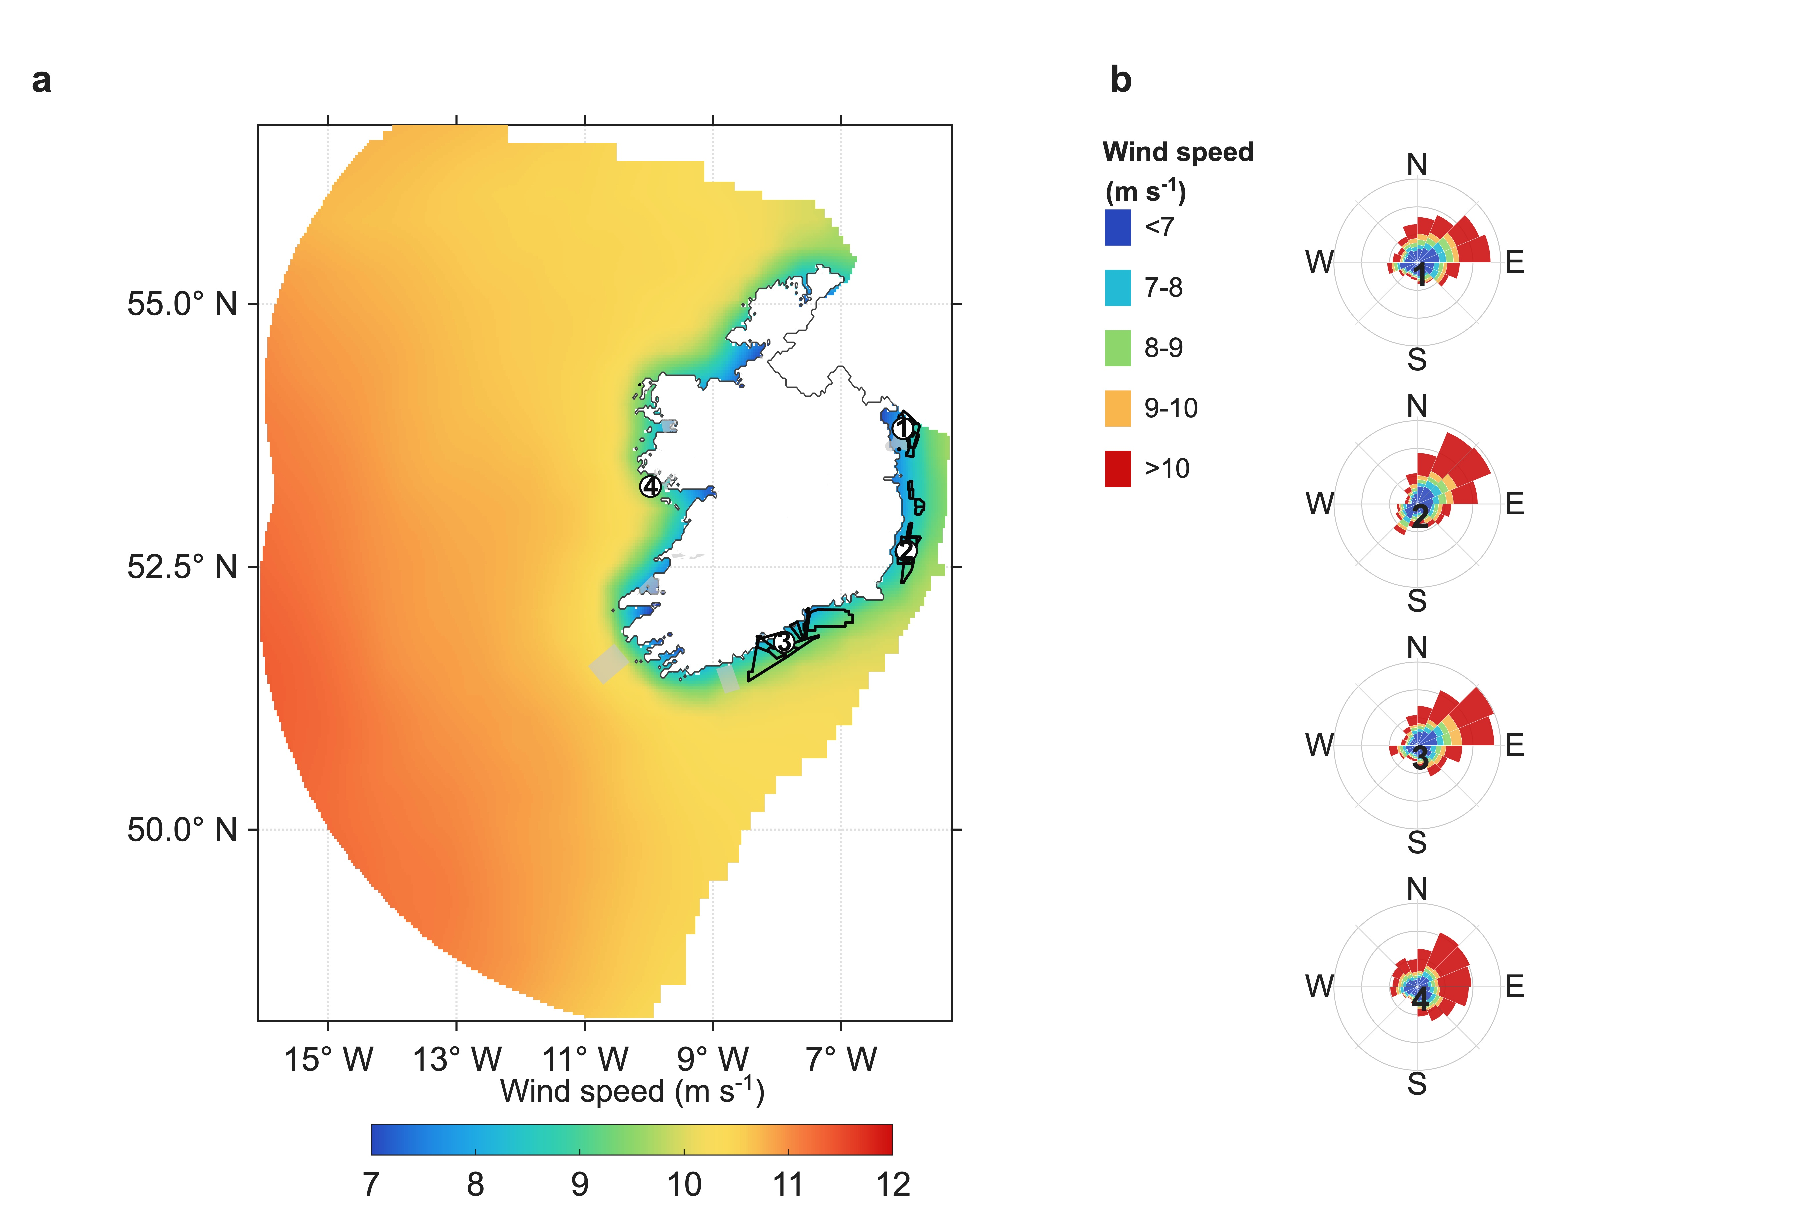
\includegraphics[width = 1\columnwidth]{figs/fig wind speed map.pdf}
    \caption{
    \textbf{Wind velocity distribution in Ireland.} 
    \textbf{a} wind speed distribution, with aquaculture sites, military areas and current and early-planning offshore wind areas overlaid;
    \textbf{b} wind roses at current and early-planning offshore wind areas, with locations marked in \textbf{a}.}
    \label{fig wind speed ireland}
\end{figure}

The ten years of historical weather data, including wind velocity, temperature, air density, etc., in the assessment areas, are collected from the ERA-5 product \cite{ERA5}. The temporal resolution is one hour, and the spatial resolution is 0.25$^\circ$ latitude and 0.25$^\circ$ longitude.
Within the grid, wind speed and other physical variables are interpolated to the assessment grid and candidate sites using bilinear interpolation.
The resulting mean wind-speed field and site-level wind-speed and wind-direction distributions are shown in Fig. \ref{fig wind speed ireland}.


\subsection{Wind turbine model}

The Vestas V236-15.0 MW offshore wind turbine is used to represent future large-scale offshore wind generation and to calculate power output as a function of wind speed \cite{V23615}. The physical parameters of the wind turbine are shown in Table \ref{tab wind turbine para}. Its power curve is shown in Fig. \ref{fig electricity curve}. When the wind speed exceeds the cut-in speed, power output increases gradually to rated power at the rated wind speed. Power output is set to zero when wind speed exceeds the cut-out speed.

\begin{table}[tbp]
\caption{Physical parameters of the Vestas V236-15.0 MW wind turbine}
\label{tab wind turbine para}
\begin{tabular}{p{1cm}p{1cm}p{1.5cm}p{1cm}p{1cm}p{2cm}p{2cm}}
\hline
Rated power & Cut-in speed & Cut-out speed & Rotor radius & Hub height & Surface roughness length & Thrust coefficient \\ \hline
15 MW       & 3 m s$^{-1}$ & 31 m s$^{-1}$ & 118 m       & 150 m      & 0.0002                   & 0.5                \\ \hline
\end{tabular}%
\end{table}

\begin{figure}
    \centering
    
\includegraphics[width = 0.8\columnwidth]{figs/fig power curve of wind turbine.pdf}
    \caption{Power-output curve of the Vestas V236-15.0 MW wind turbine}
    \label{fig electricity curve}
\end{figure}

\subsection{Wake effect}

In a wind turbine array, downstream wind speed can be reduced by upstream turbines as the incoming wind passes through the rotor blades. This is known as the wake effect, and it can reduce the power output of downstream turbines.

\begin{figure}
    \centering
    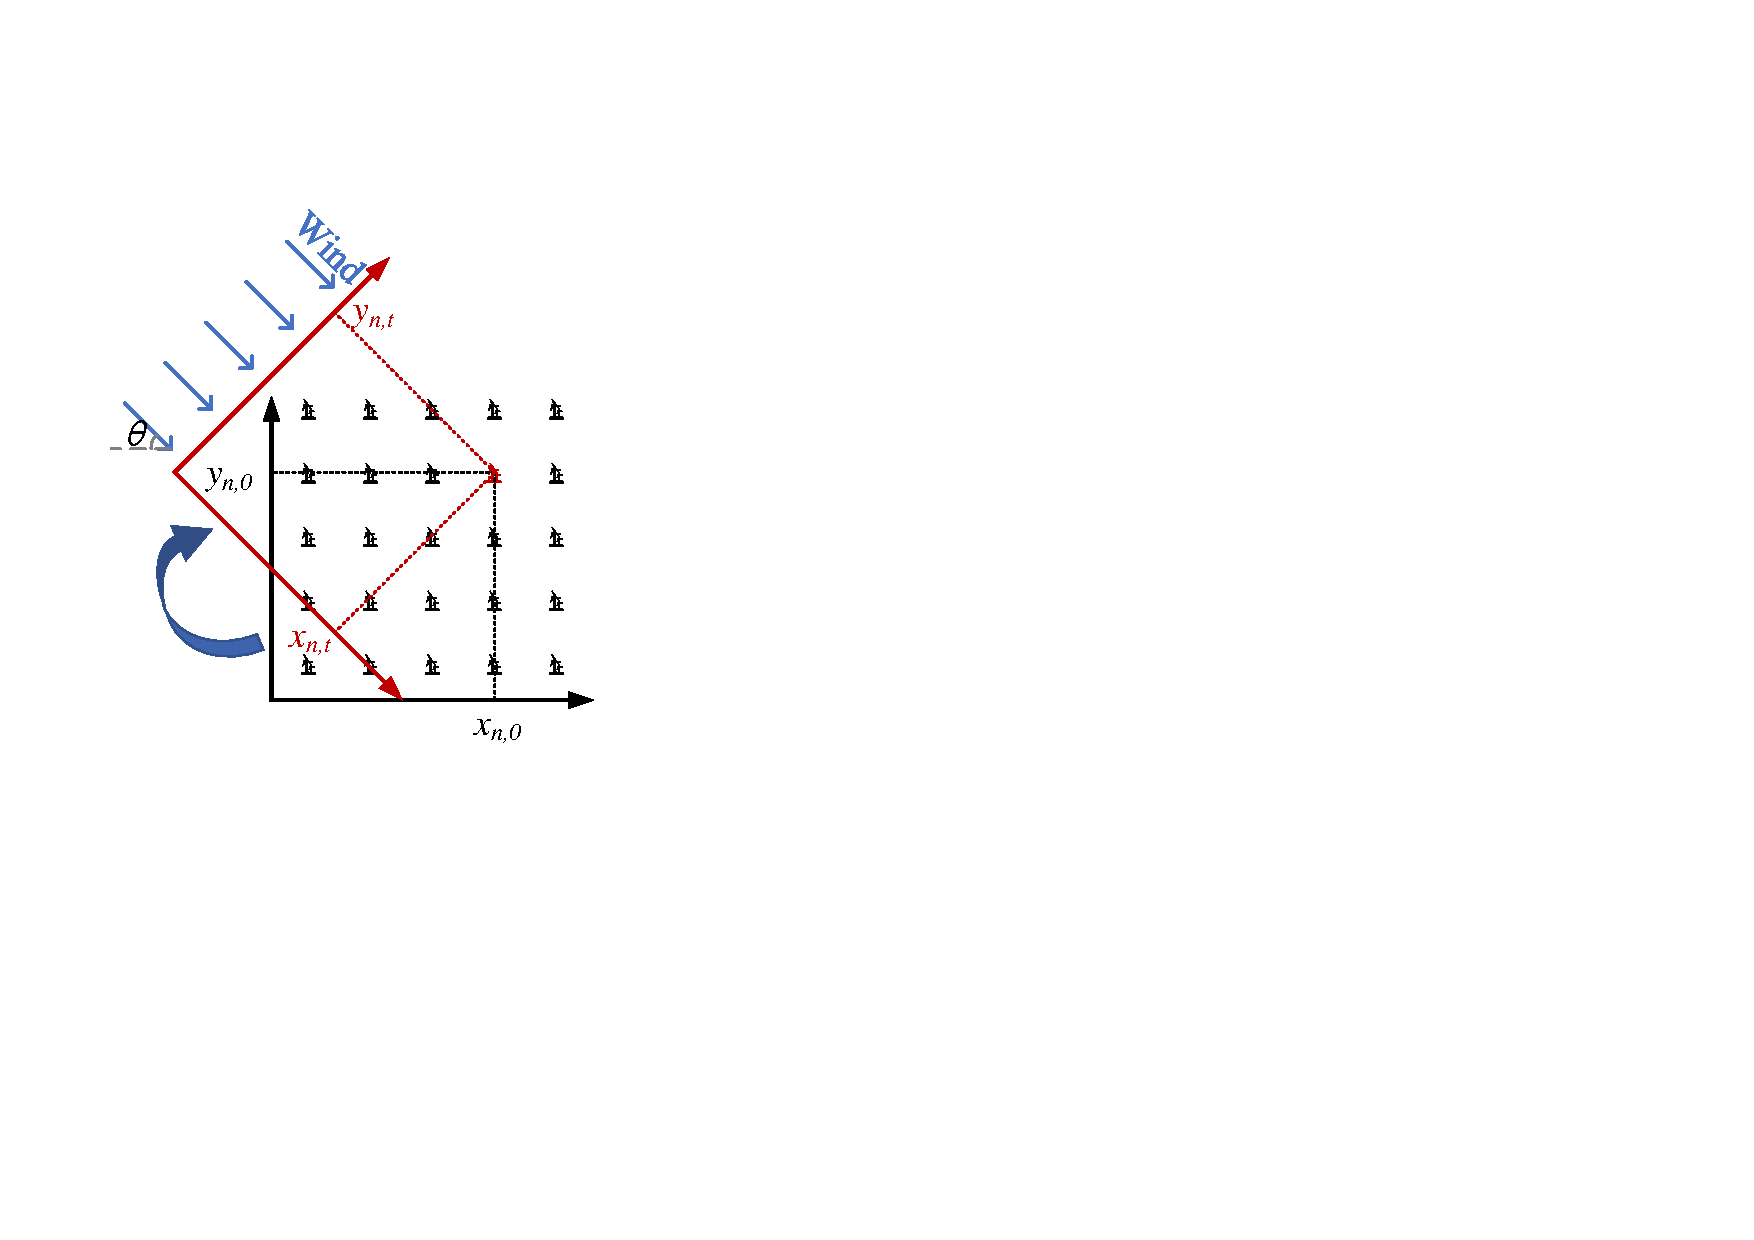
\includegraphics[width = 0.4\columnwidth]{figs/fig coordinate conversion.pdf}
    \caption{Coordinate rotation under changing wind directions}
    \label{fig coordinate rotation}
\end{figure}

The wind velocity at time $t$ is described by speed $v_t$ and direction angle $\theta_t$, measured relative to the original x-axis. To calculate wake interactions, the coordinate axes are rotated with the wind direction so that the incoming wind is parallel to the x-axis, as shown in Fig. \ref{fig coordinate rotation}. The rotated coordinates of wind turbine (WT) $n$ at time $t$, ($x'_{n,t}$,$y'_{n,t}$), are given by:
\begin{gather}
    \begin{bmatrix}
    x'_{n,t} \\
    y'_{n,t}
    \end{bmatrix}
    = 
    \begin{bmatrix}
    \cos{\theta_t} & -\sin{\theta_t} \\
    \sin{\theta_t} & \cos{\theta_t}
    \end{bmatrix}
    \begin{bmatrix}
    x_{n,0} \\
    y_{n,0}
    \end{bmatrix}
\end{gather}
where $x_{n,0}$ and $y_{n,0}$ are the original coordinates of WT $n$ before rotation.

After rotation, the wind direction is parallel to the x-axis. The wake effect is then calculated using the Jensen-Gaussian wake model. The wake-effect factor at a downstream location $(x,y)$ affected by upstream WT $n_1$ is calculated as \cite{tao2019optimal}:
\begin{align}
    f^{wake}_{n_1} = \left(1-\sqrt{1-\frac{C_T}{2 (\omega / R_{n_1} )^2}}\right) e^{-\frac{\Delta y^2}{2\omega^2}}
\end{align}
where $f^{wake}_{n_1}$ is dimensionless; the corresponding wind-speed deficit is $v_{n_1} f^{wake}_{n_1}$; $v_{n_1}$ is the wind speed at WT $n_1$; $C_T$ is the WT thrust coefficient; $R_{n_1}$ is the rotor radius; $\Delta y = |y-y_{n_1}|$ is the cross-wind distance in the rotated coordinate system; and $\omega$ is the characteristic width of the wake, calculated by \cite{tao2019optimal}:
\begin{gather}
    \omega = \left(R_{n_1} + 0.56 / (\ln{z^h} - \ln{z_0}) \Delta x \right)/2
\end{gather}
where $z^h$ is the WT hub height; $z_0$ is the surface roughness length; and $\Delta x = x-x_{n_1}, x \geq x_{n_1}$ is the downstream distance in the rotated coordinate system.

The simulation results of the Vestas V236-15.0 MW wind turbine are presented in Fig. \ref{fig wake effect simulation}. For the annual mean case, the single-turbine wake field is rotated into the fixed east--west and north--south coordinate system for each historical wind direction. Historical wind speeds are then used to convert the wake-induced wind-speed deficit into power loss, giving an annual mean wake-loss field (Fig. \ref{fig wake effect simulation}a). We also show the corresponding single-direction wake field under the worst alignment, where the downstream turbine lies on the wake centreline (Fig. \ref{fig wake effect simulation}b). In the offshore wind farm layout, we adopt a turbine spacing of $D^{wt}=2.31$ km, corresponding to 9.8 rotor diameters (9.8D) for the Vestas V236-15.0 MW turbine and consistent with the use of rotor-diameter multiples in wind-farm layout and spacing studies \cite{BurtonWindEnergyHandbook2011,MeyersMeneveau2012}. The dashed circle or dashed line marks this adopted spacing, while the solid contour marks the 5\% boundary.

\begin{figure}
    \centering
    
\includegraphics[width = 1\columnwidth]{figs/fig wake effect single.pdf}
    \caption{Wake-effect simulation around a single wind turbine. \textbf{a}, Historical annual mean wake-loss field calculated from historical wind speeds and wind directions. The dashed circle marks the adopted 2.31 km (9.8D) turbine spacing, and the solid contour marks the 5\% annual mean power-loss boundary. \textbf{b}, Single-direction wake-effect factor under the worst alignment. The dashed line marks the adopted spacing, and the solid contour marks the 5\% wake-effect-factor boundary.}
    \label{fig wake effect simulation}
\end{figure}

\section{Offshore hydrogen and other chemical products cost models}
\label{sec cost}

\subsection{Summary of several technical routes}
Several technical routes are considered in utilising the offshore wind, as shown in Fig. \ref{fig technical routes}, including:

\begin{figure}
    \centering
    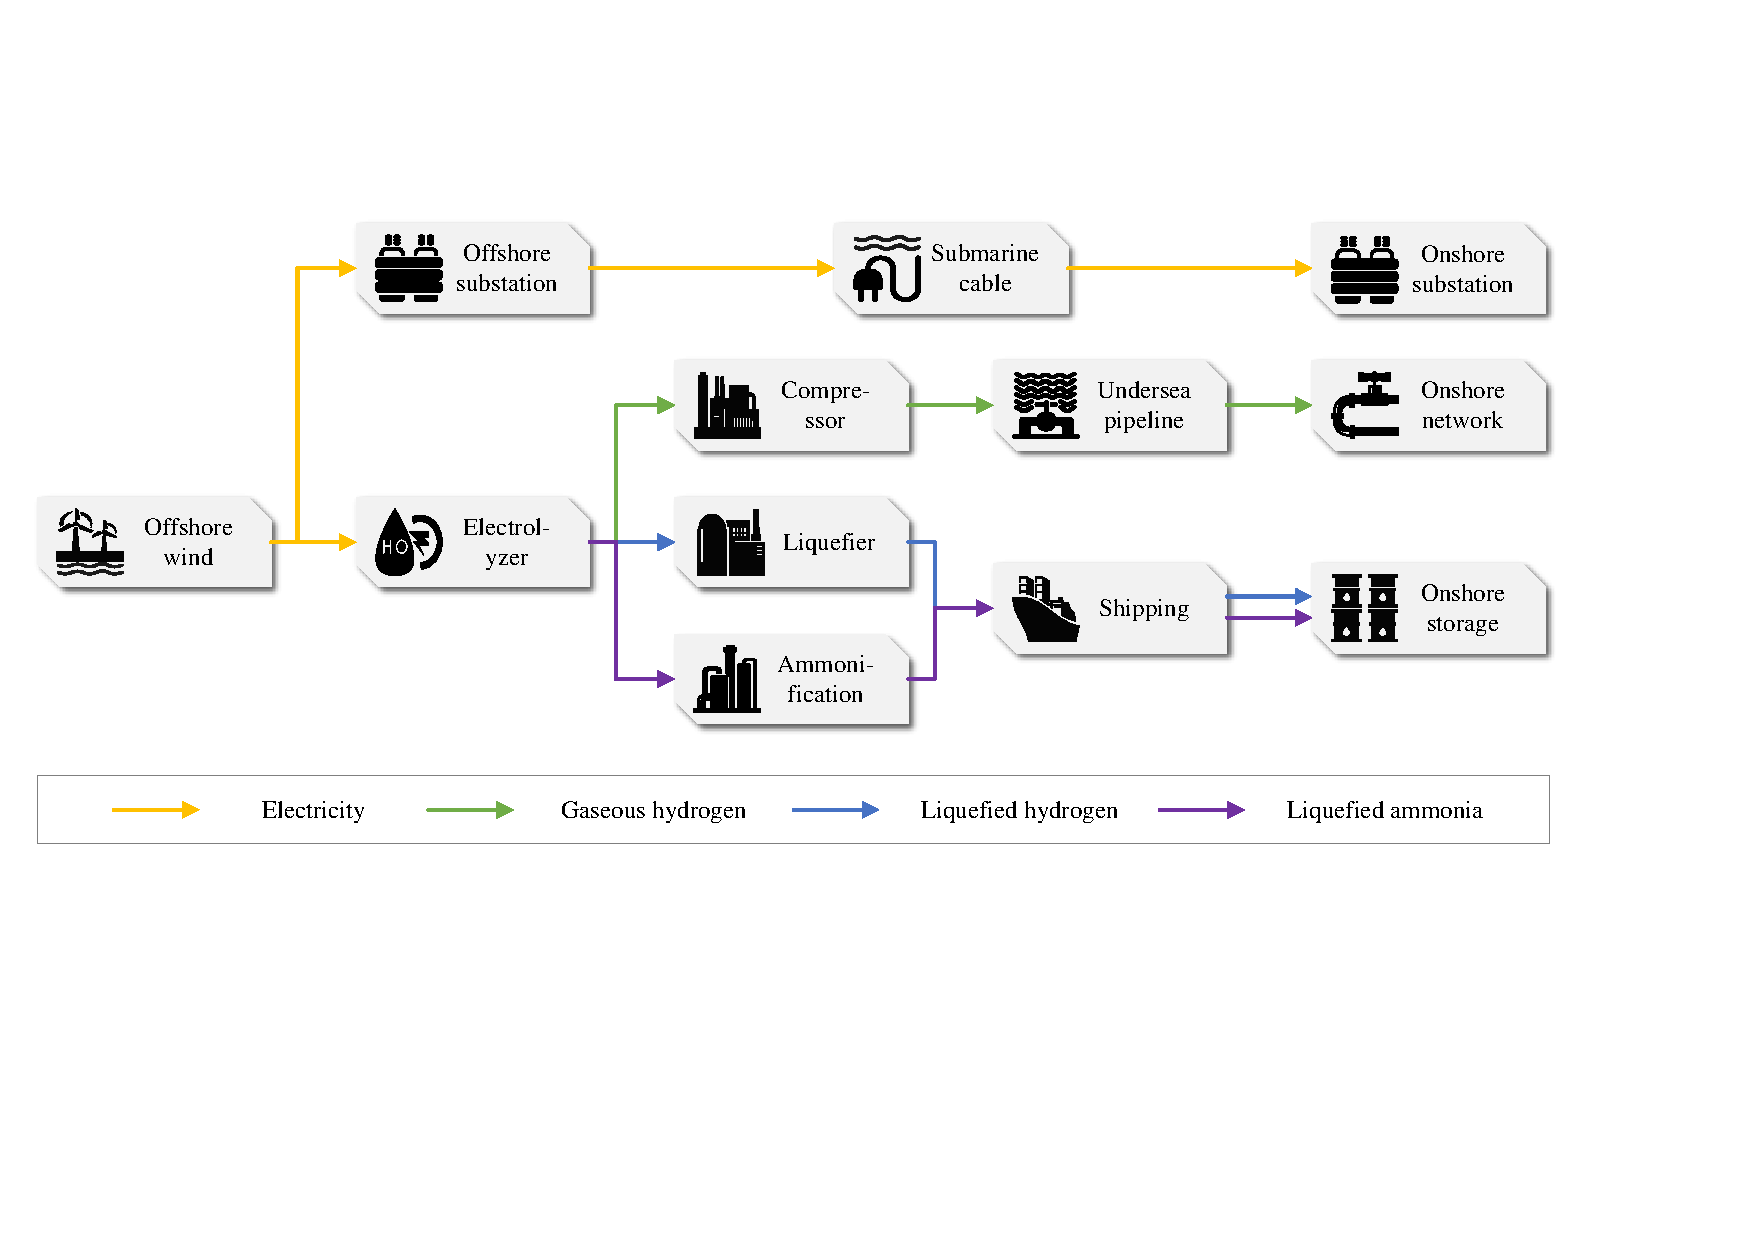
\includegraphics[width = 0.99\columnwidth]{figs/fig technical route.pdf}
    \caption{Technical routes for offshore wind utilisation}
    \label{fig technical routes}
\end{figure}

\begin{enumerate}
    \item Electricity: Offshore wind electricity is collected at an offshore substation and delivered to onshore substations through submarine cables. This route has relatively low investment cost and therefore a lower levelised cost of electricity (LCOE). However, submarine-cable length limits mean that offshore wind electricity is mainly delivered to nearby onshore power systems. The available transmission capacity also depends on onshore connection capacity, which is related to the structure and operation of the receiving power system. This domestic integration issue is analysed in Section \ref{sec domestic energy system model}.
    \item Compressed gaseous hydrogen: Green hydrogen produced by offshore electrolysers can be compressed and transported to the onshore gas system. Network transmission is cost-effective for large hydrogen volumes, but hydrogen injection into the gas network, or hydrogen blending, is limited by the allowable hydrogen molar fraction. This blending constraint affects the amount of offshore hydrogen that can be integrated into the domestic gas system. Similar to electricity transmission, undersea pipelines are also constrained by route length, so offshore hydrogen is mainly transported to nearby countries.
    \item Liquefied hydrogen: After hydrogen is liquefied, its energy density increases and it can be shipped internationally.
    \item Liquefied ammonia: Hydrogen can be further converted to ammonia through Haber--Bosch reactors. Compared with liquefied hydrogen, ammonia has a higher volumetric energy density and is therefore more suitable for long-distance and time-sensitive transport. However, if the destination cannot directly use or combust ammonia and must convert it back to hydrogen, additional cost and energy losses are introduced.
\end{enumerate}

\subsection{Route 1: electricity transmission}

The evaluation structure of LCOE of offshore wind electricity is presented in Fig. \ref{fig LCOE composition}. The total life cycle cost is divided into development expenditure (DEVEX), capital expenditure (CAPEX), operating expenditure (OPEX), and decommissioning expenditure (DECEX). They are converted into net present value to calculate the LCOE:
\begin{align}
    D^{owf} &= 8760 P^{owf,rated} CF LF T \notag\\
    LCOE &=
    \frac{DEVEX + CAPEX}{D^{owf}}
    + \frac{\sum_{t=1}^{T} OPEX_t (1+r)^{-(t-1)}}{D^{owf}}
    \notag\\
    &\quad
    + \frac{DECEX(1+r)^{-(T-1)}}{D^{owf}}
\label{eq LCOE calculation}
\end{align}
where $t$ is the index for year; $T$ is the total year of lifetime; $OPEX_t$ represents the OPEX in year $t$; $r$ is the discount rate; $P^{owf,rated}$ is the rated power of the offshore wind farm (OWF); $CF$ and $LF$ are the capacity factor and load factor of the OWF, respectively, which is calculated based on yearly simulation and historical wind data.
In the following content, each component is introduced in detail.

\begin{figure}
    \centering
    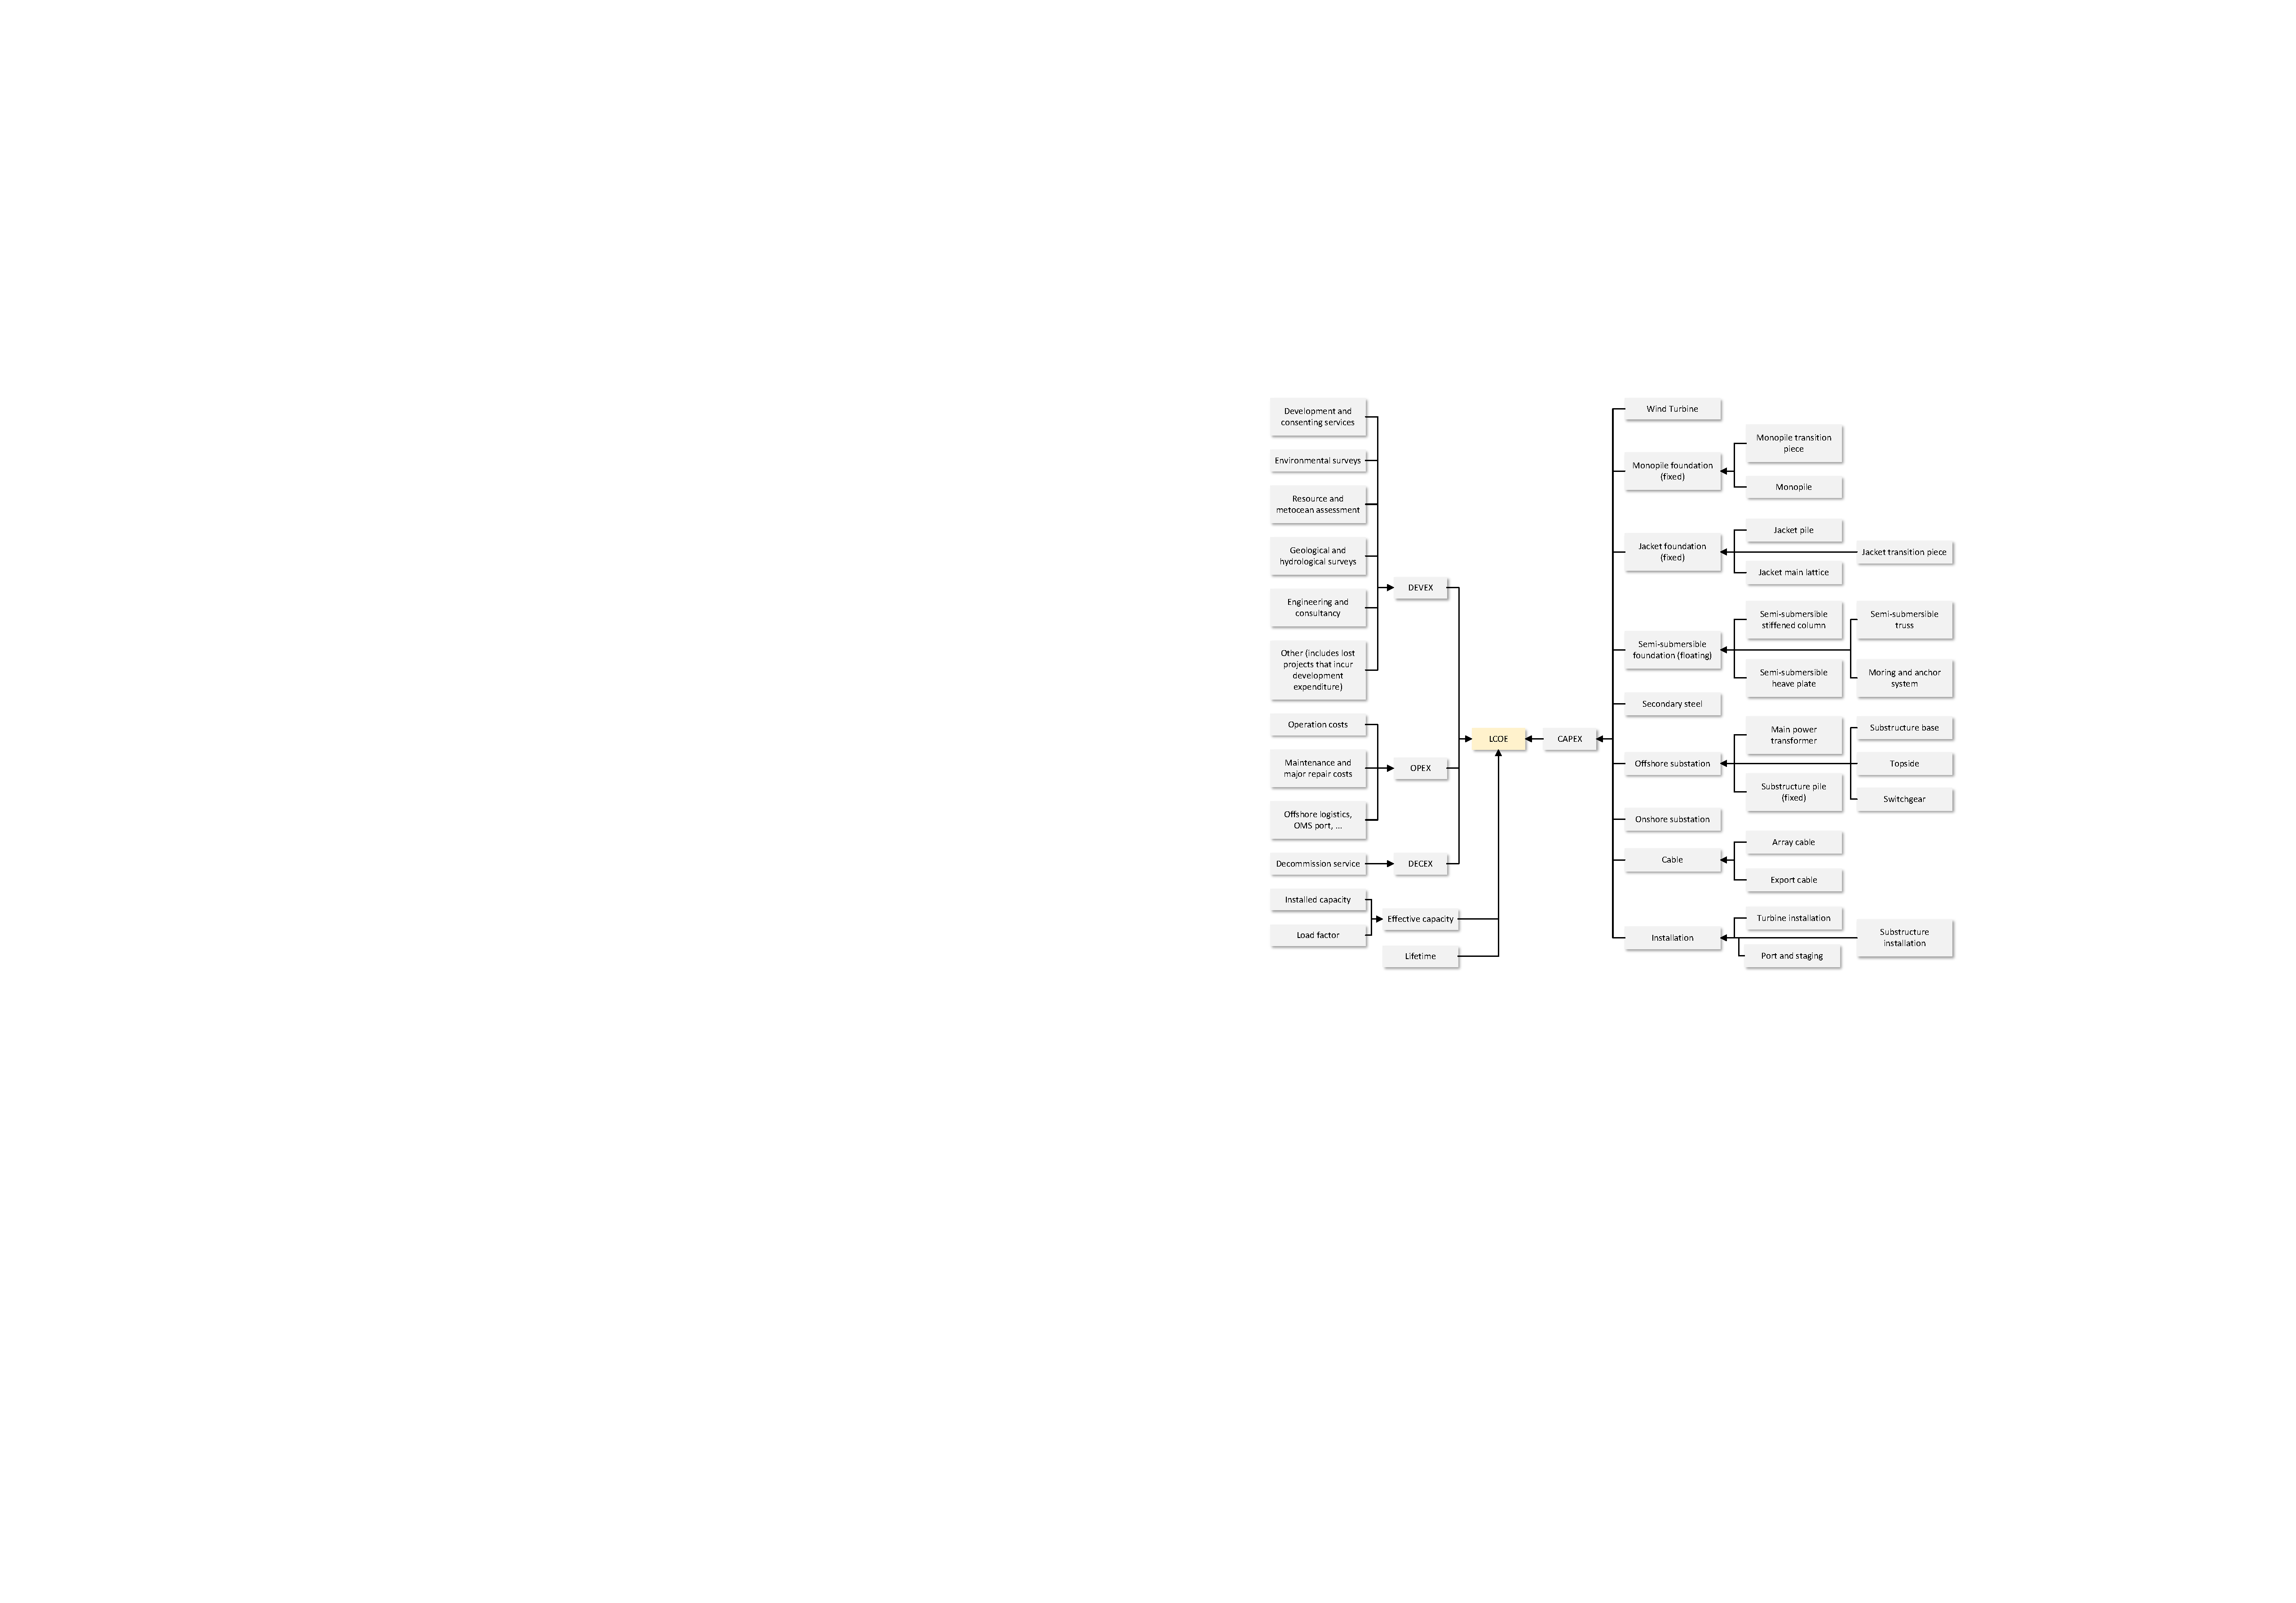
\includegraphics[width = 0.99\columnwidth]{figs/fig LCOE structure.pdf}
    \caption{Levelised-cost structure for offshore wind electricity}
    \label{fig LCOE composition}
\end{figure}

(1) DEVEX

DEVEX includes development and consenting services, environmental surveys, resource and metocean assessment, geological and hydrological surveys, engineering and consultancy, and other development costs. The data are derived from a typical reference value from a UK OWF project, as shown in Table \ref{tab devex cost} \cite{Guidetoanoffshorewindfarm}.

\begin{table}[tbp]
    \centering
    \caption{DEVEX cost items \cite{Guidetoanoffshorewindfarm}}
    \begin{tabular}{cc}
    \hline
        Items in DEVEX & Cost (\texteuro{} MW$^{-1}$)\\
    \hline
         Development and project management & 5000 \\
         Environmental survey & 4000 \\
         Resource and metocean assessment & 4000\\
         Geological and hydrological surveys & 4000\\
         Engineering and consultancy & 4000\\
         Other costs & 54000 \\
     \hline
    \end{tabular}
    \label{tab devex cost}
\end{table}

(2) CAPEX

(2.1) Wind turbine

The capital cost of wind turbines is assumed to scale linearly with rated capacity. Based on linear regression using available offshore wind project data, this relationship can be expressed for large-capacity wind turbines as \cite{dinh2023geospatial, maienza2020life}:
\begin{gather}
    C^{wt} =  (1.6 P^{wt,rated} - 1.9) \times 10^6
\end{gather}
where $C^{wt}$ is the capital cost of wind turbine, and $P^{wt,rated}$ is its rated power.

(2.2) Mono-pile foundation

Three foundations are considered: mono-pile, jacket, and semi-submersible platforms. The first two are used for fixed-bottom offshore wind. Mono-pile foundations are usually used in sandy and gravelly seabed conditions at water depths of 0--30 m, whereas jacket foundations are preferred for non-rocky seabeds at water depths of 30--60 m. Semi-submersible platforms are used for floating offshore wind in deeper offshore areas. As shown in Fig. \ref{fig water depth}, the black and red lines separate the mono-pile, jacket, and semi-submersible areas in European marine areas \cite{bathymetry2022}. Fixed-bottom platforms are usually deployed in coastal areas, but suitable areas can extend further offshore in the south-eastern North Sea near Denmark and Germany.

\begin{figure}
    \centering
    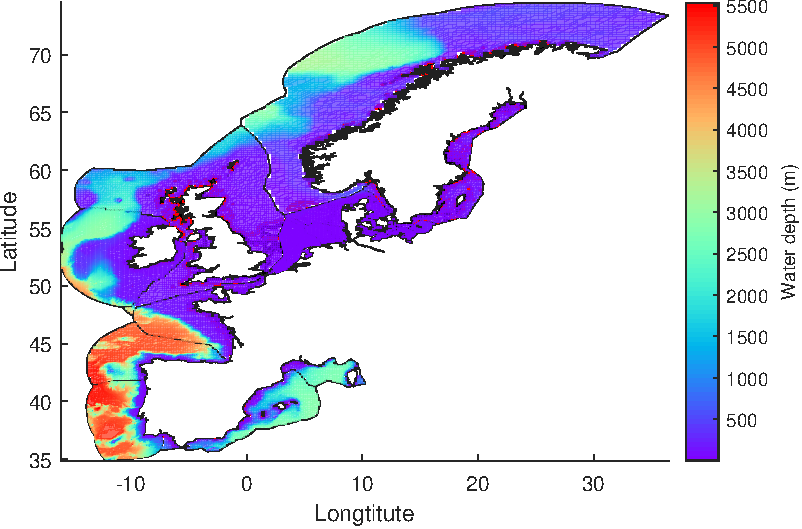
\includegraphics[width = 0.99\columnwidth]{figs/fig water depth map.pdf}
    \caption{Exclusive Economic Zone, water depth, and offshore foundation separation of coastal European countries. The black and red lines separate the marine areas that are more suitable for mono-pile, jacket, and semi-submersible platforms, respectively. Major coastal countries are analysed in this paper (including Belgium (BE), Denmark (DK), France (FR), Germany (DE), Ireland (IE), Netherlands (NL), Norway (NO), Portugal (PT), Spain (ES), Sweden (SE), and the UK (GB)). }
    \label{fig water depth}
\end{figure}

Mono-pile foundation includes the mono-pile structure and transition piece, where the capital cost is calculated based on the mass used in the structure. The mass is fitted based on data in recently committed offshore wind projects \cite{NRELOffshoreBalance}:
\begin{gather}
    M^{mono-pile} = 10^{-4} \bigg( (10^3 P^{wt,rated})^{1.5} + 10^{-1}(H^{wt})^{3.7} 
\notag \\
    + 2100(H^{wd})^{2.25} + (10^3 M^{rna})^{1.13} \bigg)
\\
    M^{mono-trans} = e^{2.77 + 1.04(P^{wt,rated})^{0.5} + 0.00127(H^{wd})^{1.5}}
\end{gather}
where $M^{mono-pile}$ and $M^{mono-trans}$ are the masses of mono-pile and transition piece, respectively; $P^{wt,rated}$ is the rated power of the wind turbine; $H^{wt}$ is the hub height; $H^{wd}$ is the water depth; $M^{rna}$ is the rotor nacelle assembly mass, which can be calculated as:
\begin{gather}
    M^{rna} = 2.082 (P^{wt,rated})^2 + 44.59 P^{wt,rated} + 22.48
\end{gather}

Then, the capital cost of the mono-pile foundation can be calculated by:
\begin{gather}
    C^{mono} = \rho^{mono-pile} M^{mono-pile} + \rho^{mono-trans} M^{mono-trans}
\end{gather}
where $\rho^{mono-pile}$ and $\rho^{mono-trans}$ are the cost rates of mono-pile and transition piece materials. The material cost rates (\texteuro{} ton$^{-1}$) are fitted from offshore wind project cost data points in the UK \cite{Guidetoanoffshorewindfarm}:

(2.3) Jacket foundation

The mass of the jacket foundation (including the main lattice, transition piece, and pile), $M^{jacket-ml}$, $M^{jacket-tp}$, and $M^{jacket-pile}$, can be calculated as \cite{NRELOffshoreBalance}:
\begin{gather}
    M^{jacket-ml} = e^{3.71 + 0.00176(P^{wt,rated})^{2.5} + 0.645\ln \left( {(H^{wd})}^{1.5}\right)}
\\
    M^{jacket-tp} = 
    \left( \frac{-0.0131+0.0381}{\ln{P^{wt,rated}}} -2.27\times 10^{-9} (H^{wd})^3 \right)^{-1} 
\\
    M^{jacket-pile} = 8 e^{0.5574 \left(3.71 + 0.00176(P^{wt,rated})^{2.5} + 0.645\ln \left( {(H^{wd})}^{1.5}\right)\right)}
\end{gather}

Then, the total cost of the jacket foundation can be calculated as:
\begin{align}
    C^{jacket} = & \rho^{jacket-ml} M^{jacket-ml} + \rho^{jacket-tp} M^{jacket-tp} 
    \notag\\
    & + \rho^{jacket-pile} M^{jacket-pile}
\end{align}
where $\rho^{jacket-ml}$, $\rho^{jacket-tp}$, and $\rho^{jacket-pile}$ are the cost rates of the main lattice, transition piece, and pile of jacket foundation, respectively.

(2.4) Semi-submersible foundation

The semi-submersible foundation includes a stiffened column, truss, heave plate, and mooring and anchor system. The masses of the stiffened column, truss and heave plate are denoted as $M^{semi-sc}$, $M^{semi-tr}$, and $M^{semi-hp}$, respectively, and can be calculated as \cite{NRELOffshoreBalance,gonzalez2024techno}:
\begin{align}
    M^{semi-sc} = -0.9571(P^{wt,rated})^2 + 40.89(P^{wt,rated}) + 802.09
\\
    M^{semi-tr} = 2.7894 (P^{wt,rated})^2 + 15.591 P^{wt,rated} + 266.03
\\
    M^{semi-hp} = - 0.4397 (P^{wt,rated})^2 + 21.545 P^{wt,rated} + 177.42
\end{align}
The total semi-submersible structural mass is:
\begin{gather}
    M^{semi} = M^{semi-sc} + M^{semi-tr} + M^{semi-hp}
\end{gather}

Additionally, the cost of mooring and anchor system $C^{mo}$ can be calculated as:
\begin{align}
    C^{mo} = N^{wt} N^{lin} (C^{anc} + (1.5 H^{wd} + 410) C^{lin} + 50 C^{ch})
\end{align}
where $N^{wt}$ is the number of wind turbines; $N^{lin}$ is the number of mooring lines per turbine or floater (assumed to be 4 in this study); $C^{anc}$ is the cost of an individual anchor; $C^{lin}$ and $C^{ch}$ are the cost of each mooring line and chain sector per unit of length, respectively.

Then, the cost of the semi-submersible foundation $C^{semi}$ can be calculated as:
\begin{gather}
    C^{semi} = \rho^{semi-sc} M^{semi-sc} + \rho^{semi-tr} M^{semi-tr} + \rho^{semi-hp} M^{semi-hp} + C^{mo}
\end{gather}
where $\rho^{semi-sc}$, $\rho^{semi-tr}$, and $\rho^{semi-hp}$ are the cost rates of the semi-submersible stiffened column, truss, and heave plate, respectively.

(2.5) Secondary steels

Secondary steel refers to the steel used to support the ladders, railings, walkways, etc. The mass of these materials depends on different foundation structures. For a fixed structure, the mass $M^{scd-fx}$ can be calculated as in (\ref{eq secondary steel fixed}); for a semi-submersible foundation, it can be calculated as in (\ref{eq secondary steel semisubmersible}) \cite{NRELOffshoreBalance}:
\begin{gather}
    M^{scd-fx} = 40 + \left(0.8\left(18+H^{wd}\right)\right)
\label{eq secondary steel fixed} \\
    M^{scd-semi} = -0.153(P^{wt,rated})^2 + 6.54 P^{wt,rated} + 128.34
\label{eq secondary steel semisubmersible}
\end{gather}
The corresponding secondary-steel costs are:
\begin{gather}
    C^{scd-fx} = \rho^{scd} M^{scd-fx} \\
    C^{scd-fl} = \rho^{scd} M^{scd-semi}
\end{gather}
where $\rho^{scd}$ is the secondary-steel cost rate.

(2.6) Offshore substation

The offshore substation mainly consists of electrical facilities (main power transformers, switchgear for HVDC transportation) and supporting structures (topside structures, foundation platforms and bottom piles). 

The total capacity of the main power transformers must match the OWF capacity. A 20\% redundancy margin is used \cite{guo2023grid}. The number of main power transformers is calculated as:
\begin{align}
    N^{mpt} = \lceil{1.2 P^{owf,rated} /  P^{mpt,rated}}\rceil
\end{align}
where $P^{mpt,rated}$ = 300 MVA is the capacity of the main power transformer. 

The switchgear isolates and protects the key electrical equipment and helps with the conversion of voltage. It contains high-voltage and mid-voltage ones, whose number matches the number of the main power transformer, i.e., $N^{switchgear} = N^{mpt}$.

The topside structure of the substation contains the spaces in the offshore substation. The mass of topside structure $M^{offsub-top}$ is also fitted from the project data, with respect to the properties of main power transformers \cite{NRELOffshoreBalance}:
\begin{align}
    M^{offsub-top} = 3.85 (P^{mpt,rated} N^{mpt}) + 285
\end{align}

Other substation foundation structures depend on the type of OWF. For fixed structure, the mass of substation foundation $M^{offsub-fdt-fx}$ can be calculated as:
\begin{gather}
    M^{offsub-fdt-fx} = 40 + (0.8(18+H^{wd}))
\end{gather}

For floating one, the mass $M^{offsub-fdt-fl}$ can be calculated as:
\begin{gather}
    M^{offsub-fdt-fl} = 2(M^{semi} + M^{scd-semi})
\end{gather}

Specifically for fixed foundations, the mass of the supporting pile can be calculated as:
\begin{gather}
    M^{offsub-pile} = 8 (M^{offsub-fdt-fx})^{0.5574}
\end{gather}

Then, the capital cost of the offshore substation can be added up as follows. 
For fixed structure, the cost $C^{offsub-fx}$ can be calculated as:
\begin{gather}
    C^{offsub-fx} = \rho^{mpt} P^{mpt,rated} N^{mpt} + (\rho^{switch-hv} 
\notag\\
    + \rho^{switch-mv}) N^{switchgear} + \rho^{offsub-top} M^{offsub-top}
    \notag\\
    + \rho^{offsub-fdt-fx} M^{offsub-fdt-fx} + \rho^{offsub-pile} M^{offsub-pile}
\end{gather}
where $\rho^{mpt}$, $\rho^{switch-hv}$, $\rho^{switch-mv}$, $\rho^{offsub-top}$, $\rho^{offsub-fdt-fx}$, and $\rho^{offsub-pile}$ are the unit costs of main power transformer, high-voltage and medium-voltage switchgear, topside materials, fixed foundation, and supporting pile, respectively.

For floating structure, the cost $C^{offsub-fl}$ can be calculated as:
\begin{gather}
    C^{offsub-fl} = \rho^{mpt} P^{mpt,rated} N^{mpt} + (\rho^{switch-hv} 
\notag\\
    + \rho^{switch-mv}) N^{switchgear} + \rho^{offsub-top} M^{offsub-top}
\notag\\
    + \rho^{offsub-fdt-fl} M^{offsub-fdt-fl}
\end{gather}
where $\rho^{offsub-fdt-fl}$ is the unit cost of the floating foundation.

(2.7) Onshore substation

The onshore substation cost $C^{onsub}$ can be calculated as:
\begin{gather}
    C^{onsub} = 11652(V_i+P^{owf,rated}) + 1.2 \times 10^6
\end{gather}
where $V_i$ is the voltage level at the interconnection point of the offshore wind.

(2.8) Submarine cables

The submarine cables can be divided into export cables and array cables, where array cables merge the power generation of the wind turbine to the offshore substation, and export cables transport the electricity to the onshore substation.
The number of array cables $N^{cb-ar}$ is calculated from the rated powers of the cables and wind turbines, with a margin reserved for redundancy \cite{guo2023grid}. The array cable layout is approximated by the shortest connection path, so the number of links between wind turbines is approximately equal to the number of wind turbines. Then, we have:
\begin{gather}
    N^{cb-ar} = N^{wt} \lceil 1.1 P^{wt,rated} / P^{cb-ar,rated} \rceil
\end{gather}
where $P^{cb-ar,rated}$ is the rated power of the candidate array cables.

The cost of the array cable depends on the length of each array cable, which is further related to the structure of the wind turbines. For fixed foundation:
\begin{gather}
    C^{cb-ar-fx} = 0.1 \sqrt{P^{cb-ar,rated}} N^{cb-ar} \times 1.1 (D^{wt}+2H^{wd}) 
\end{gather}
where $D^{wt}$ is the distance between wind turbines, set to 2.31 km (9.8D) as described in Section \ref{sec offshore wind farm model}.

For floating structures:
\begin{gather}
    C^{cb-ar-fl} = 0.1 \sqrt{P^{cb-ar,rated}} N^{cb-ar} \times 1.1 (2H^{wd}/\cos{(\theta^{hg})} + D^{wt})
\end{gather}
where $\theta^{hg}$ is the hanging angle, which can be calculated by \cite{NRELOffshoreBalance}:
\begin{gather}
    \theta^{hg} = (-0.0047H^{wd}+18.743)/180\times \pi
\end{gather}

Similarly, the number of export cables is calculated based on the total capacity of the OWF:
\begin{gather}
    N^{cb-ex} = \lceil 1.1 P^{owf,rated} / P^{cb-ex,rated} \rceil
\end{gather}

Then, the costs of export cable for fixed and floating structures can be calculated as (\ref{eq cost export cable fixed}) and (\ref{eq cost export cable floating}), respectively:
\begin{gather}
    C^{cb-ex-fx} =  0.1 \sqrt{P^{cb-ex,rated}} N^{cb-ex} \times 1.1 (2 H^{wd} + D^{cn})
\label{eq cost export cable fixed} \\
    C^{cb-ex-fl} =  0.1 \sqrt{P^{cb-ex,rated}} N^{cb-ex} \times 1.1 (2 H^{wd}/\cos{(\theta^{hg})} + D^{cn})
\label{eq cost export cable floating} 
\end{gather}
where $D^{cn}$ is the distance between the OWF and the nearest connection point, which can be calculated as:
\begin{gather}
    D^{cn} = \min_{i \in \mathcal{I}^{E}} ||x^{owf}-x_i, y^{owf}-y_i||_2
\label{eq distance to power bus}
\end{gather}
where $i$ is the index for the electric bus; $\mathcal{I}^{E}$ is the set of all the electric buses; coordinate $x_i$ and $y_i$ represent the longitude and latitude of electric bus $i$, and $x^{owf}$ and $y^{owf}$ are the longitude and latitude of the OWF, respectively.

(2.9) Installation cost

The installation cost consists of three parts: substructure installation cost, turbine installation cost, and port/staging cost. They are fitted based on recently committed OWF project data, which can be found in \cite{ASpatialEconomic}.
Summarising all capital cost items and the installation cost, the CAPEX can be calculated depending on the structure of the OWF. The mono-pile, jacket, and semi-submersible types of offshore wind are calculated in (\ref{eq capex mono}), (\ref{eq capex jacket}), and (\ref{eq capex semi}), respectively.
\begin{gather}
    CAPEX = N^{wt} \left( C^{wt} + C^{mono} + C^{scd-fx} + C^{cb-ar-fx} \right) + C^{offsub-fx} \notag\\
    + C^{onsub} + C^{cb-ex-fx} + C^{int}
\label{eq capex mono} \\
    CAPEX = N^{wt} \left( C^{wt} + C^{jacket} + C^{scd-fx} + C^{cb-ar-fx} \right) + C^{offsub-fx} 
    \notag\\
    + C^{onsub} + C^{cb-ex-fx} + C^{int}
\label{eq capex jacket} \\
    CAPEX = N^{wt} \left( C^{wt} + C^{semi} + C^{scd-fl} + C^{cb-ar-fl} \right) + C^{offsub-fl} 
    \notag\\
    + C^{onsub} + C^{cb-ex-fl} + C^{int}
\label{eq capex semi}
\end{gather}
where $C^{int}$ is the installation cost.

(3) OPEX

The OPEX includes the operation and maintenance costs. The yearly cost is mainly related to the distance of the OWF to the nearest port. This relationship is also derived based on committed project data \cite{ASpatialEconomic}. For fixed OWF, we have (\ref{eq opex fixed}); for floating one, we have (\ref{eq opex floating}).
\begin{gather}
    OPEX_t = (2.5522 \ln(D^{port}) + 90.899) \times 10^6
\label{eq opex fixed}\\
    OPEX_t = (4.0739 \ln(D^{port}) + 76.993) \times 10^6
\label{eq opex floating}
\end{gather}
where the locations of major ports in Europe can be found in \cite{EMODnet}, as presented in Fig. \ref{fig distance to port}.


\begin{figure}
    \centering
    
\includegraphics[width = 0.99\columnwidth]{figs/fig distance to port.pdf}
    \caption{Distance to the nearest major port across the modelled European EEZs. Dots denote the aggregated major port locations used in the cost model.}
    \label{fig distance to port}
\end{figure}

(4) DECEX

The DECEX is assumed to be proportional to the installation cost. The value of the proportion $\alpha$ is derived from recent UK projects \cite{Guidetoanoffshorewindfarm}. It can be calculated as:
\begin{gather}
    DECEX = \alpha^{decex} C^{int}
\end{gather}
where $\alpha^{decex}$ is the decommissioning factor.

\subsection{Route 2: hydrogen production}

\begin{figure}
    \centering
    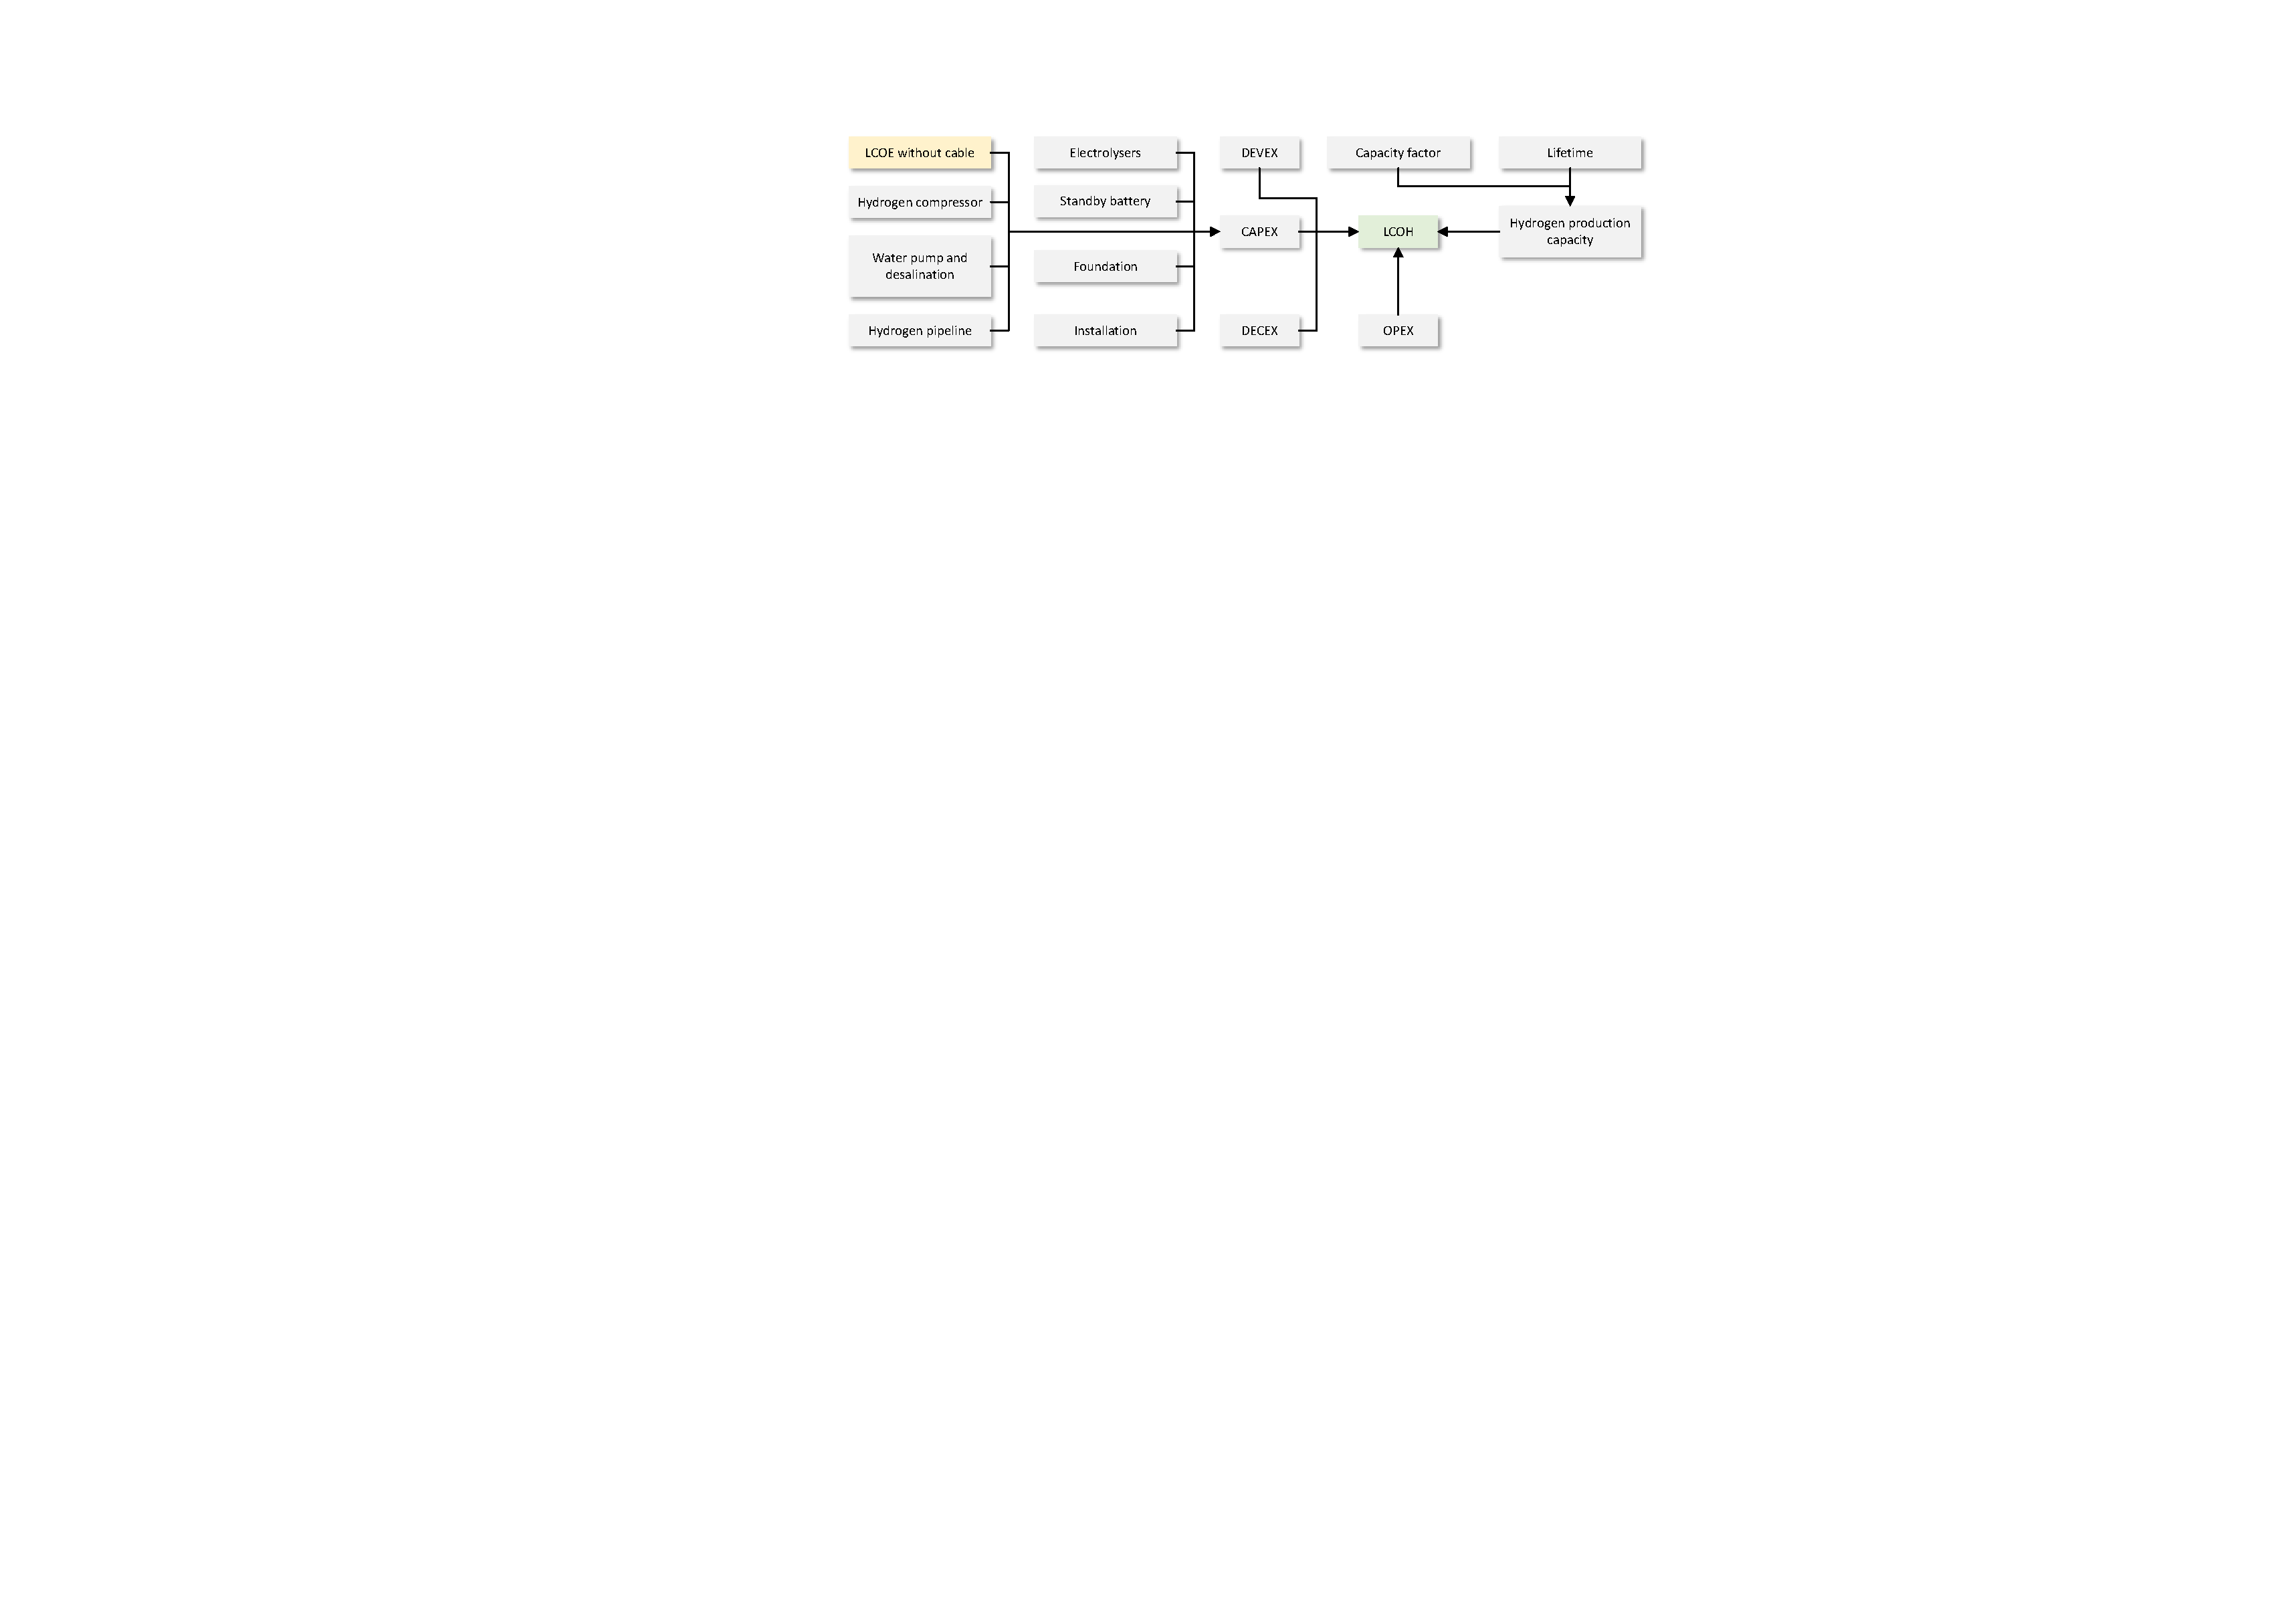
\includegraphics[width =1\columnwidth]{figs/fig LCOH structure.pdf}
    \caption{Cost structure of offshore hydrogen production.}
    \label{fig lcoh structure}
\end{figure}

The LCOH calculation structure is shown in Fig. \ref{fig lcoh structure}. It follows the same levelised-cost structure as (\ref{eq LCOE calculation}), with additional offshore hydrogen-production components and their associated expenditures.

On the offshore electrolysis platform, wind-generated electricity is consumed by electrolysis, water pumping and desalination, hydrogen compression, and standby battery losses. These energy flows are modelled as:
\begin{gather}
    P^{el} \eta^{el} = Q^{hy} HV^{hy}
\label{eq electrolyser efficiency} \\
    P^{wpd} = \eta^{wpd} M^{water}
\label{eq electricity consumption water pump desal}    \\
    P^{cp} = \eta^{cp} Q^{hy} \left( (p^{hy,high}/p^{hy,low})^{Z^{hy}(1-1/\beta^{cp})}-1 \right)
\label{eq electricity consumption compressor}    \\
    P^{bt} = (1-\eta^{bt}) UL^{bt} (P^{el} + P^{wpd} + P^{cp})
\label{eq battery loss}    \\
    P^{bt} + P^{el} + P^{wpd} + P^{cp} = P^{owf,rated} \times CF
\label{eq electricity consumption total}
\end{gather}
where (\ref{eq electrolyser efficiency}) represents the electrolysis conversion process; (\ref{eq electricity consumption water pump desal}) links water-pumping and desalination power to the processed water mass; (\ref{eq electricity consumption compressor}) gives the compressor power consumption \cite{bao2019multi}; (\ref{eq battery loss}) evaluates standby battery losses; and (\ref{eq electricity consumption total}) enforces the total platform power balance. $P^{el}$, $P^{wpd}$, $P^{cp}$, and $P^{bt}$ represent the power consumption or loss of the electrolyser, water pumping/desalination system, compressor, and battery, respectively. $\eta^{el}$, $\eta^{wpd}$, $\eta^{cp}$, and $\eta^{bt}$ are the corresponding efficiencies; $Q^{hy}$ is the hydrogen production flow rate under standard temperature and pressure; $HV^{hy}$ is the heat value of hydrogen; $M^{water}$ is the processed water mass; $p^{hy,low}$ and $p^{hy,high}$ are the hydrogen pressures before and after compression; $Z^{hy}$ is the hydrogen compressibility factor; $\beta^{cp}$ is the specific heat ratio; and $UL^{bt}$ is the battery utilisation rate.

The resulting hydrogen production flow is then used to calculate LCOH as:
\begin{align}
    D^{hy} &= 8760 Q^{hy} HV^{hy} LF T \notag\\
    LCOH &=
    \frac{DEVEX + CAPEX}{D^{hy}}
    + \frac{\sum_{t \in \mathcal{T}} OPEX_t (1+r)^{-(t-1)}}{D^{hy}}
    \notag\\
    &\quad
    + \frac{DECEX(1+r)^{-(T-1)}}{D^{hy}}
\end{align}

As for LCOE, the total expenditure for offshore hydrogen production includes DEVEX, CAPEX, OPEX, and DECEX. Because the offshore wind-farm expenditure is already included in the LCOE calculation, this subsection focuses on the additional hydrogen-system costs.

\begin{table}[tbp]
\centering
\caption{Additional offshore hydrogen-system cost assumptions \cite{OffshoreWindandHydrogen, Offshorewindtogreen}}
\label{tab offshore hydrogen system cost}
\begin{tabular}{llll}
\hline
Capital cost                                                                                                    & Cost in 2030 & Cost in 2040 & Cost in 2050 \\ \hline
Alkaline electrolyser ($10^3$ \texteuro{} MW$^{-1}$)                       & 625          & 400          & 300          \\
Hydrogen compressor ($10^3$ \texteuro{} MW$^{-1}$)                         & 3.86         & 2.69         & 2.34         \\
Battery ($10^3$ \texteuro{} MW$^{-1}$)                                       & 56.39        & 41.54        & 22.58        \\
Water desalination ($10^3$ \texteuro{} MW$^{-1}$)                            & 1.4          & 0.936        & 0.234        \\
Platform ($10^3$ \texteuro{} MW$^{-1}$)                                      & 232.13       & 195.98       & 130.45       \\
System replacement ($10^3$ \texteuro{} MW$^{-1}$)                            & 10.96        & 21.11        & 11.49        \\
Pipeline ($10^3$ \texteuro{} (km $\times$ inch)$^{-1}$)       & 34.74        & 31.42        & 28.41        \\ \hline
\multicolumn{2}{l}{Operation   \& maintenance cost}                                                                               &              &              \\ \hline
Alkaline electrolyser ($10^3$ \texteuro{} MW$^{-1}$ yr$^{-1}$)                  & 12.5         & 8            & 6            \\
Hydrogen compressor ($10^3$ \texteuro{} MW$^{-1}$ yr$^{-1}$)                   & 0.117        & 0.0819       & 0.0351       \\
Battery ($10^3$ \texteuro{} MW$^{-1}$ yr$^{-1}$)                                 & 1.4          & 1.04         & 0.56         \\
Water desalination ($10^3$ \texteuro{} MW$^{-1}$ yr$^{-1}$)                    & 0.0468       & 0.0234       & 0.0117       \\
Platform ($10^3$ \texteuro{} MW$^{-1}$ yr$^{-1}$)                                & 2.92         & 2.92         & 2.92         \\
Pipeline ($10^3$ \texteuro{} (km $\times$ inch)$^{-1}$ yr$^{-1}$) & 1.0423       & 0.9427       & 0.8525       \\ \hline
\end{tabular}
\end{table}

The capital and operation and maintenance costs of the alkaline electrolyser, hydrogen compressor and other hydrogen-system components are listed in Table \ref{tab offshore hydrogen system cost}. Hydrogen pipeline cost is calculated from the minimum distance between the offshore substation and onshore gas buses, similar to (\ref{eq distance to power bus}). Installation and maintenance costs are normalised using the offshore wind-farm cost equations described above and therefore depend on the distance to the nearest port. Decommissioning expenditure is taken as the same proportion of installation cost.
% Moreover, the produced oxygen during the electrolysis process is considered a by-product and sold to onshore consumers (such as hospitals) \cite{song2021production}.

\subsection{Route 3: ammonia production}

In Route 3, offshore hydrogen from Route 2 is further converted into ammonia for liquid-product transport. We therefore add the capital, operation and maintenance, and decommissioning cost terms associated with the air-separation and Haber-Bosch synthesis units, following \cite{gonzalez2024techno}. The resulting levelised ammonia cost is reported on a hydrogen-equivalent energy basis, so that hydrogen and ammonia options can be compared consistently in the cost-supply curve and trade model.

\subsection{Cost-supply curves and future cost trends}

Water depth and distance to port are shared spatial cost drivers for the offshore electricity, hydrogen and ammonia routes. Fig. \ref{fig water depth distribution} compares their distributions across the studied EEZs. Belgium is concentrated in the lower-left part of the distribution because its potential offshore locations are relatively shallow and close to ports, whereas potential offshore locations in Spain and Norway generally have deeper water and longer port distances. These spatial differences affect installation, maintenance and support-structure costs, and therefore influence the resulting levelised costs for electricity, hydrogen and ammonia.

\begin{figure}
    \centering
    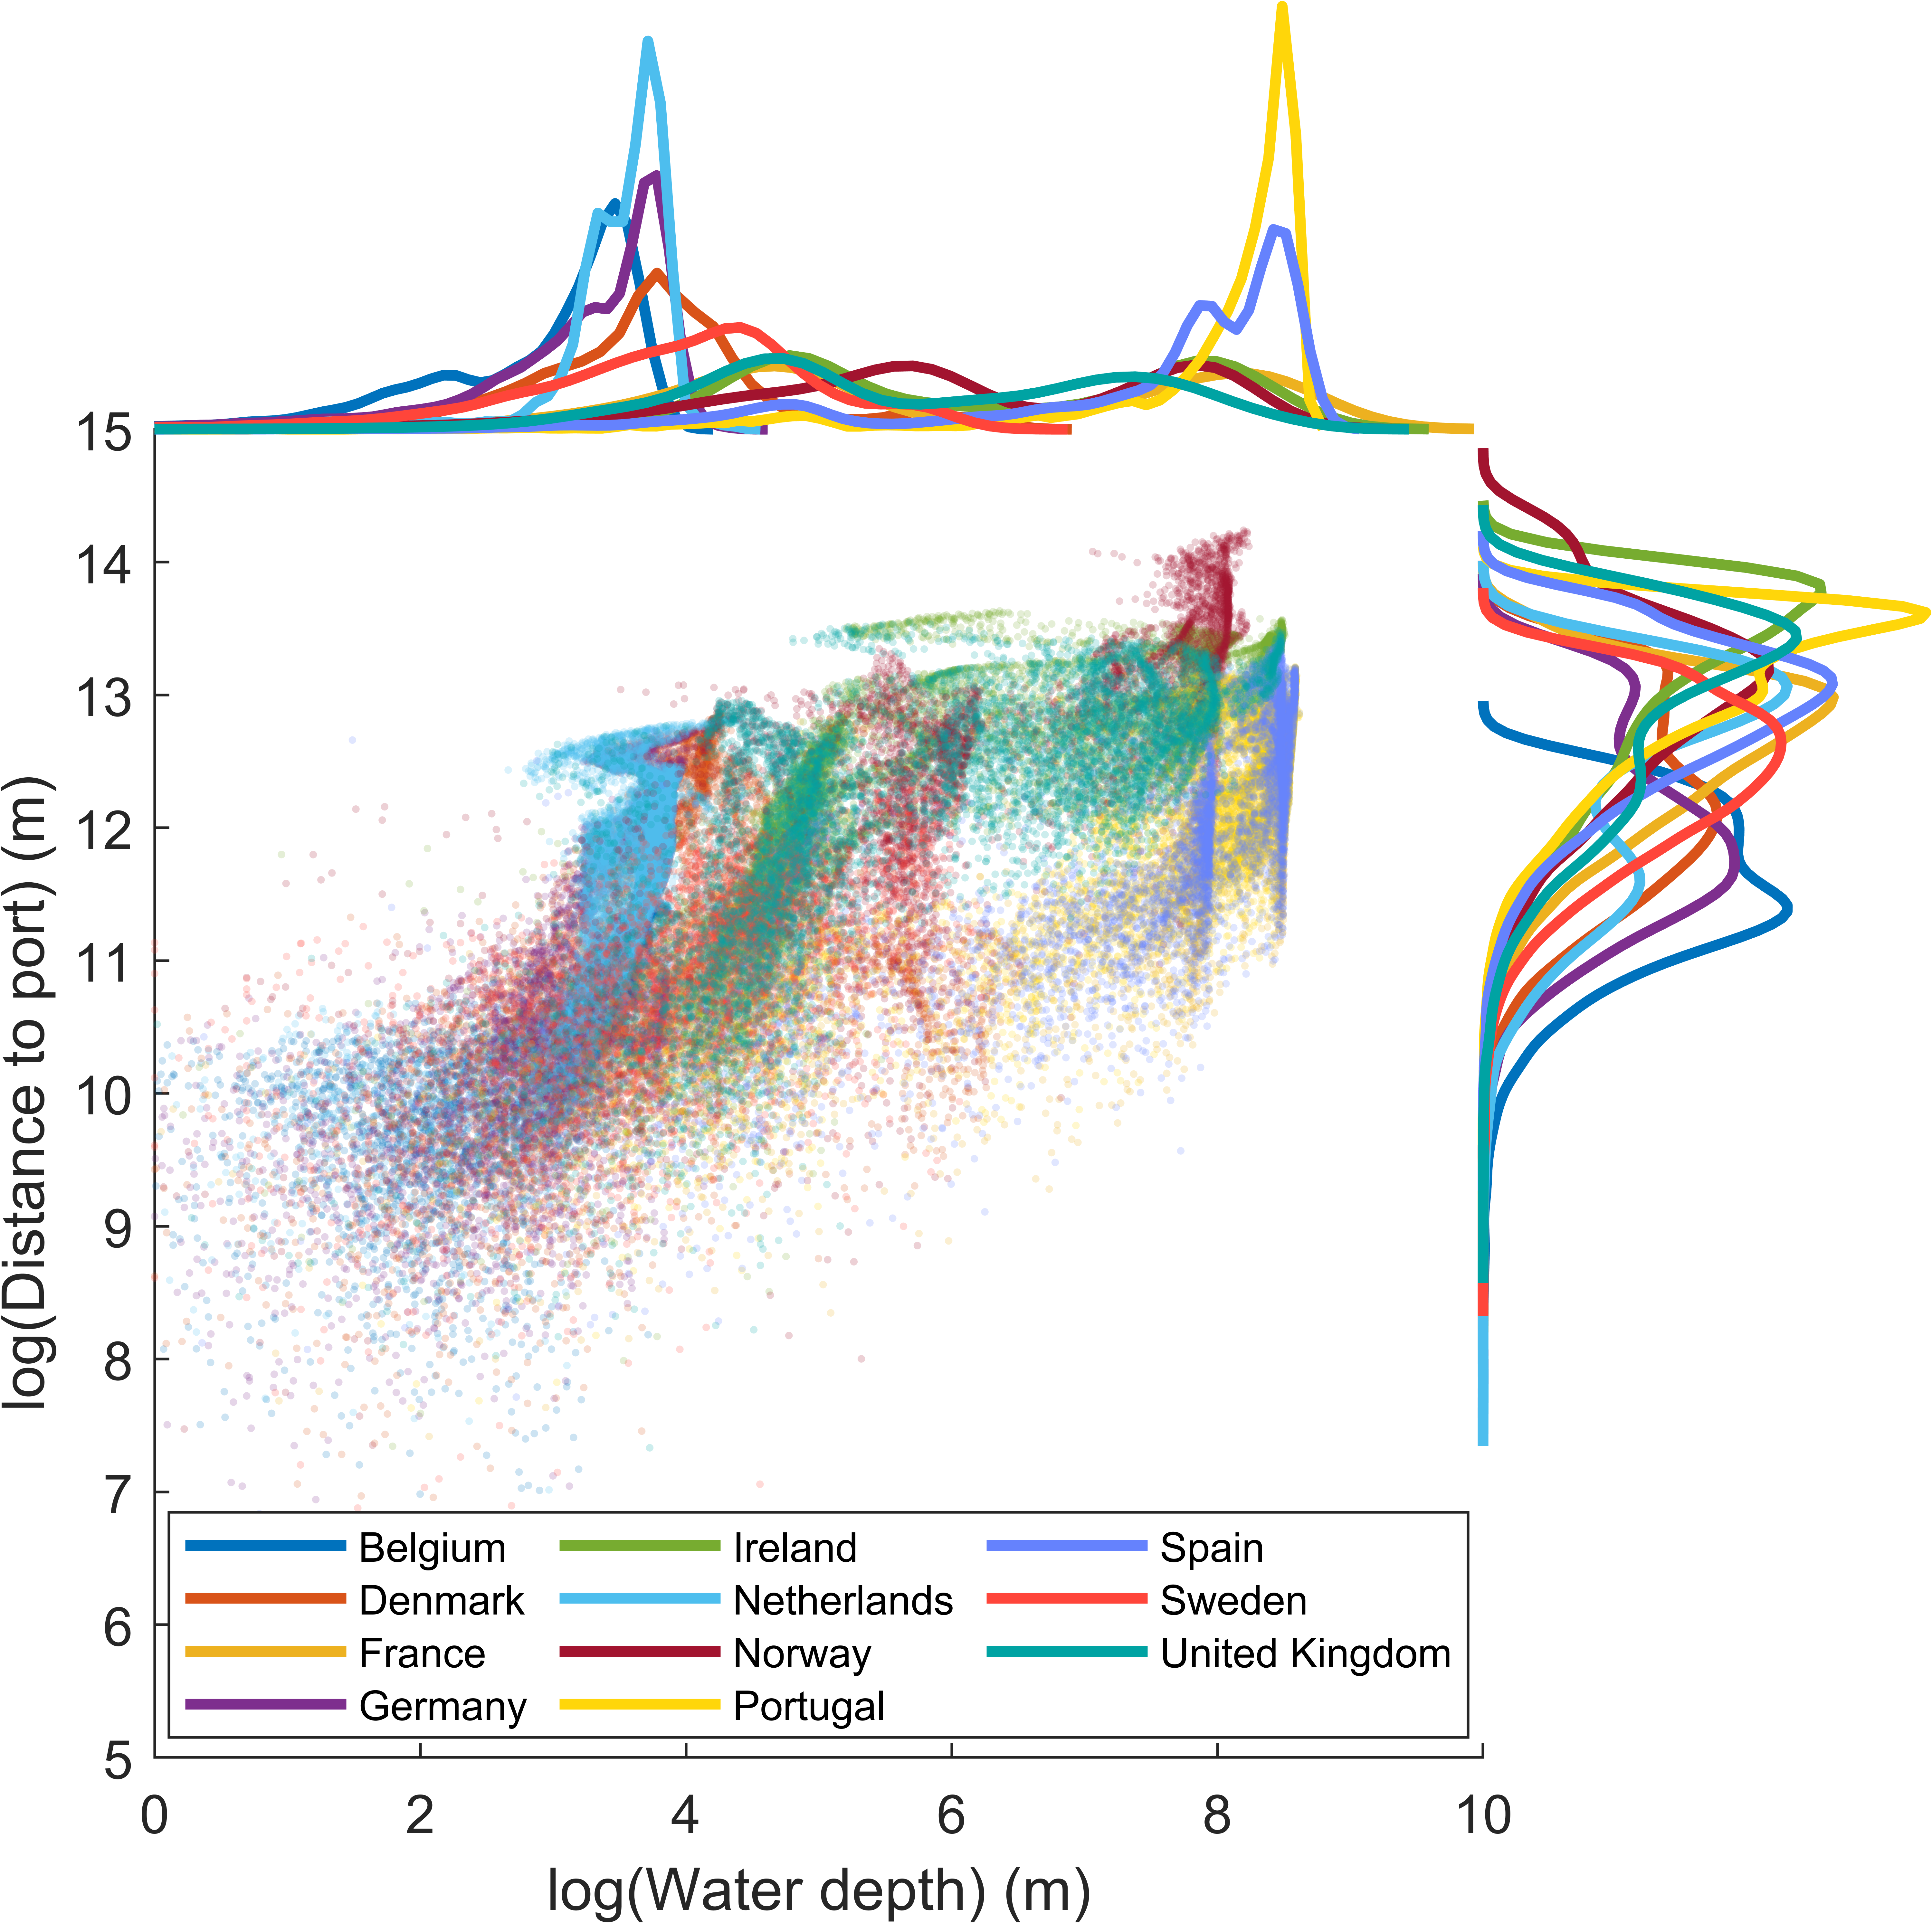
\includegraphics[width =1\columnwidth]{figs/fig distribution of water depth and distance to port.png}
    \caption{Spatial cost drivers for offshore electricity, hydrogen and ammonia cost-supply curves. The side panels show the distributions of water depth and distance to the nearest major port for each studied country, and the centre panel shows the corresponding offshore candidate locations.}
    \label{fig water depth distribution}
\end{figure}

Based on the spatially resolved levelised-cost maps, country-level cost-supply curves are derived by combining each grid cell's levelised cost with its deployable production capacity. Power density determines how much offshore wind capacity can be installed within each available area. Wake effects, as analysed in Supplementary Section 2.3, set an upper limit for power density because closely spaced turbines interfere with downstream turbines. Areas excluded from offshore wind deployment, such as military areas and aquaculture sites, are assigned zero power density. In deployment-constrained areas, power density is further reduced with increasing vessel density to reserve space for shipping lanes and other marine uses, as shown in Fig. \ref{fig vessel and power density}.
Marine areas in the southern North Sea, including parts of the EEZs of Belgium and neighbouring countries, have high vessel density. Therefore, even where water depth and distance to port are favourable, the quantity of low-cost hydrogen and ammonia supply can be limited by lower deployable power density.
The right-hand panels of Fig. \ref{fig vessel and power density} show the resulting power-density distributions across each country's EEZ. For most of Belgium's EEZ, power density is around 2.5--3.5 MW km$^{-2}$ because of the busy shipping lanes. Denmark, Germany and the Netherlands show similar constraints. In contrast, Ireland and the UK have higher power-density modes, around 4--5 MW km$^{-2}$, because vessel density is lower in large parts of their offshore areas, especially along the western coasts.

\begin{figure}
    \centering
    \includegraphics[width = 0.99\columnwidth]{figs/fig vessel density and power density.png}
    \caption{Vessel density and deployable offshore wind power density. The left panel shows vessel-density constraints used to reduce deployable power density, and the right panels show the resulting power-density distributions across each country's EEZ.}
    \label{fig vessel and power density}
\end{figure}

\begin{figure}
    \centering
    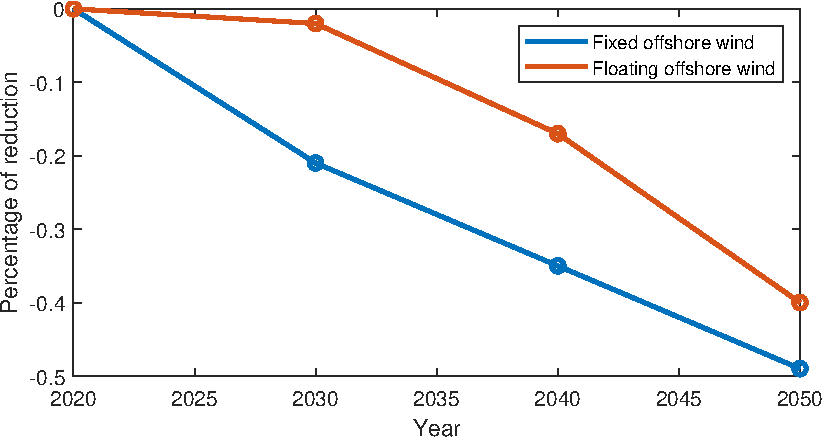
\includegraphics[width = 0.8\columnwidth]{figs/fig cost reduction.pdf}
    \caption{Assumed offshore wind cost-reduction trajectories for fixed-bottom and floating offshore wind.}
    \label{fig cost reduction}
\end{figure}

Future cost-supply curves for 2030, 2040 and 2050 are derived by applying offshore wind LCOE reduction assumptions \cite{wiser2021expert} and the hydrogen-system capital-cost assumptions in Table \ref{tab offshore hydrogen system cost}. Under the median cost-reduction scenario shown in Fig. \ref{fig cost reduction}, fixed-bottom offshore wind costs decline by 21\%, 35\% and 49\% relative to 2020 in 2030, 2040 and 2050, respectively, while floating offshore wind costs decline by 2\%, 17\% and 40\% over the same years.

\section{Domestic energy system optimisation model}
\label{sec domestic energy system model}

\begin{figure}
    \centering
    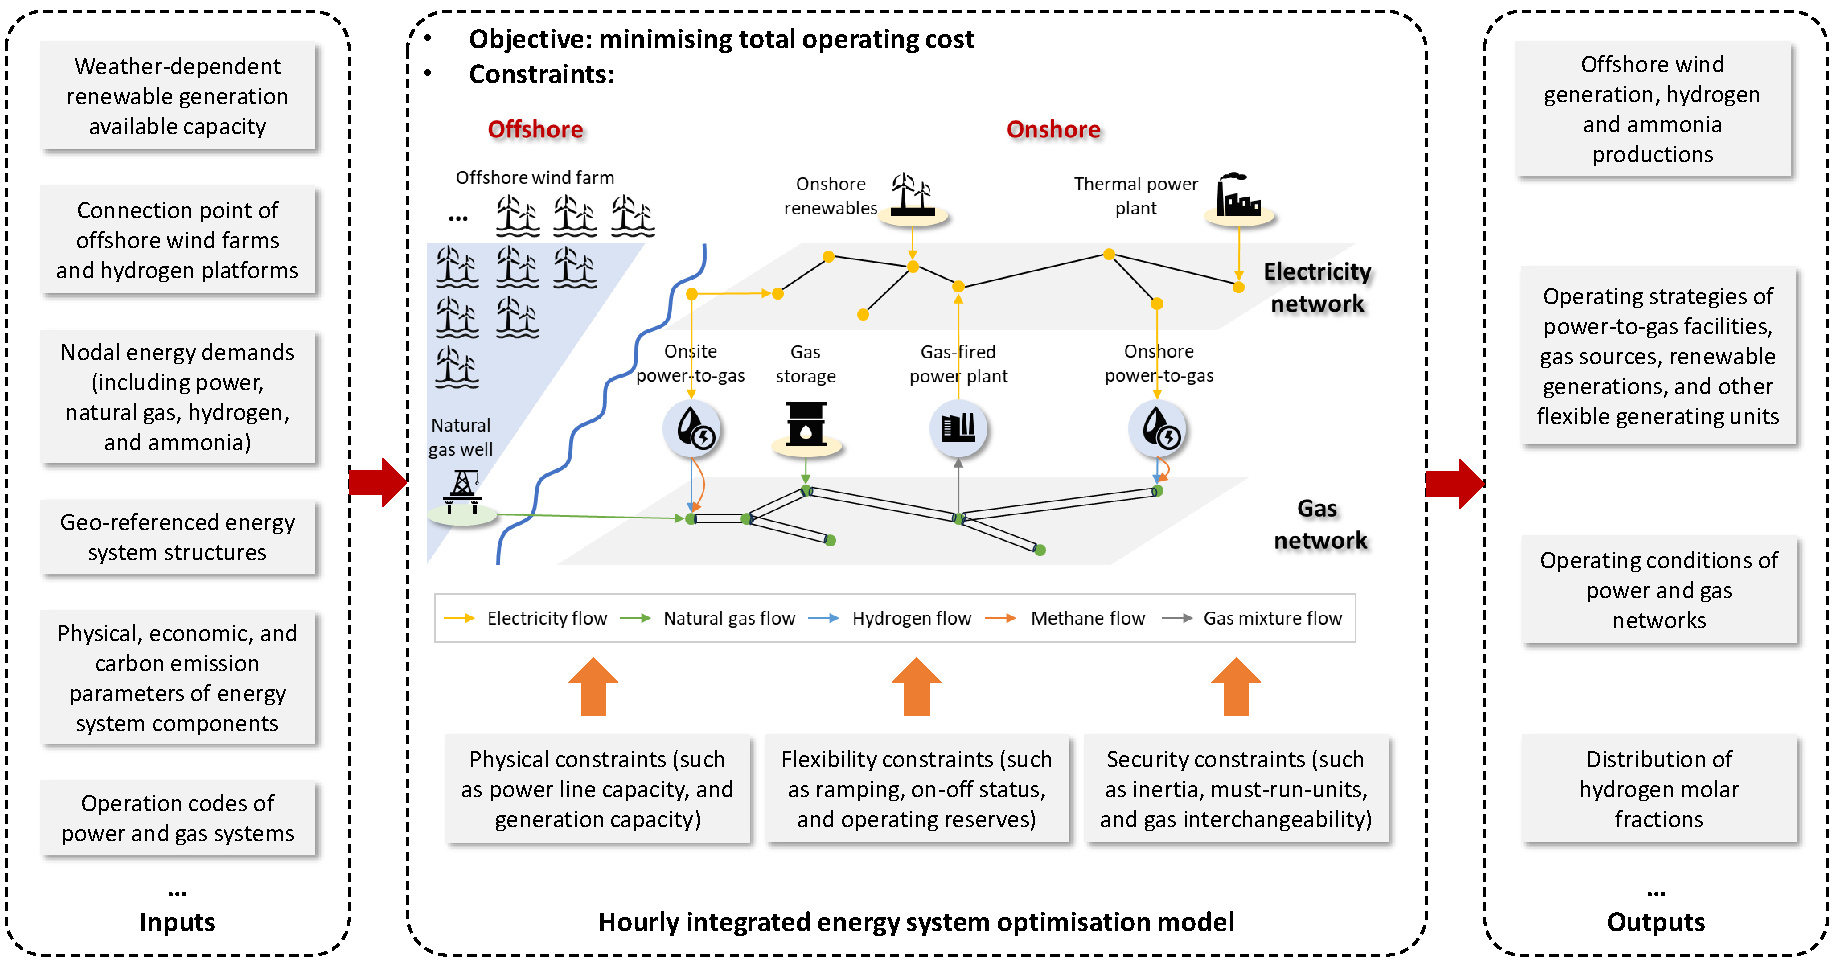
\includegraphics[width = 0.99\columnwidth]{figs/fig optimization structure.pdf}
    \caption{Framework of the integrated power--gas system operation model for domestic offshore wind and hydrogen integration.}
    \label{fig optimization framework}
\end{figure}

This section describes the domestic energy-system operation model used to evaluate how offshore wind and hydrogen production can be integrated into the All-Ireland power and gas systems before the remaining hydrogen is available for export.
The framework is shown in Fig. \ref{fig optimization framework}.
The optimisation is solved at hourly resolution over one year, while offshore wind inputs are represented on a $0.1^{\circ}\times 0.1^{\circ}$ longitude--latitude grid across the Irish offshore wind assessment areas.
All-island energy systems, including the power and gas systems in the Republic of Ireland and Northern Ireland, are within the scope of this study. The power and gas systems are coupled by gas-fired power plants and power-to-gas facilities, allowing bidirectional energy exchange and expanding the flexible operating region. Different hydrogen blending ratios are represented in the 2030, 2040, and 2050 scenarios.

The objective of the optimisation problem is to minimise the total operating cost $C^{op}$ during daily scheduling and operation, including power-system fuel and start-up costs and gas-system supply costs:
\begin{align}
    C^{op} & = \sum_{h \in \mathcal{H}} \bigg( \sum_{i \in \mathcal{I}^e} \sum_{g \in \mathcal{G}_i} \left[ u^{on}_{i,g,h} (a_{i,g} P_{i,g,h}^2 + b_{i,g} P_{i,g,h} + c_{i,g}) + u_{i,g,h}^{up} \rho^{up}_{i,g} \right]
    \notag \\
    & + \sum_{i \in \mathcal{I}^g} \rho_{i}^{gs} Q_{i,h}^{gs} \bigg)
\end{align}
where $h$, $i$, and $g$ are the indices for hours, electricity/gas nodes, and generators, respectively; $\mathcal{H}$, $\mathcal{G}$, $\mathcal{I}^e$, and $\mathcal{I}^g$, are the set of hours, generators, electricity nodes, and gas nodes, respectively; $u^{on}_{i,g,h}$ is the status of the generator $g$ at node $i$ in hour $h$, where 1 means on, and 0 means off; $u_{i,g,h}^{up}$ is the start-up action of generators, where 1 means the action is taken, and 0 indicates otherwise;
$a_{i,g}$, $b_{i,g}$, and $c_{i,g}$ are the generator cost coefficients, which depend on fuel type, fuel price and heat efficiency obtained from the Single Electricity Market (SEM) Committee \cite{SEMPLEXOS}; these parameters are provided as piecewise functions and fitted into quadratic form for convex optimisation; $P_{i,g,h}$ is the power output of the generator; $\rho^{up}_{i,g}$ is the start-up cost; $\rho_{i}^{gs}$ is the natural gas purchasing price; $Q_{i,h}^{gs}$ is the flow rate of gas supply.

\subsection{Power system model}

The schematic diagram of the All-Ireland power system is presented in Fig. \ref{fig Ireland power system}. The January 2022 network model contains 370 buses above 110 kV, 686 branches, and 155 onshore transmission-connected generators, with a total generating capacity of 19.55 GW. Daily electricity peak-demand projections to 2032 are obtained from the bottom-up forecast in EirGrid's Ten-Year Generation Capacity Statement \cite{GenerationCapacity}, covering typical seasonal scenarios (winter, summer, and spring--autumn). Because the annual growth trend in power demand is relatively steady, an Autoregressive Integrated Moving Average (ARIMA) model is used to fill the missing values between 2033 and 2050. The 15-minute-resolution electricity and gas demand curves are obtained from EirGrid's smart grid dashboard and the Gas Networks Ireland data dashboard \cite{SmartGridDashboard, GasconsumptionbyMarketSector}. For the hourly optimisation model, each hourly demand value is calculated as the average of the four corresponding 15-minute values.

\begin{figure}
    \centering
    
\includegraphics[width = 0.99\columnwidth]{figs/fig ireland power system2.pdf}
    \caption{All-Ireland transmission-network topology at 400 kV, 275 kV, 220 kV and 110 kV, redrawn from EirGrid's TYTFS bus and circuit records \cite{AllIslandTenYear}.}
    \label{fig Ireland power system}
\end{figure}

(1) Generators

According to the fuels used for generation, the generators in the Irish power system include coal, gas, gas oil, waste, peat, hydro, wind, and solar units. Detailed technical, economic, and carbon-emission-related data are obtained from the Single Electricity Market (SEM) Committee and EirGrid \cite{SEMPLEXOS, AllIslandTenYear}. The generators are divided into three categories: non-gas fossil-fuel units, gas-fired units, and renewable generators. The fuel supplies of non-gas fossil-fuel units depend on their own supply chains, which are treated as stable. Their capacity constraints are given by (\ref{eq nongas generator capacity}). The fuel supply of gas-fired units depends on the operating status of the gas system, as represented by (\ref{eq gas generator capacity}). The available output of renewable generators depends on weather conditions, and their capacity constraints are given by (\ref{eq renewable generator capacity}). Wind speed and solar radiation are obtained from the ERA-5 dataset \cite{ERA5}. Equation (\ref{eq generator on-off}) describes the on-off constraint of generators.
\begin{gather}
    u_{i,g,h}^{on} P_{i,g}^{min} \leq P_{i,g,h} \leq u_{i,g,h}^{on} P_{i,g}^{max}, g \in \mathcal{G}_i^{coal,gasoil,waste,peat}
\label{eq nongas generator capacity} \\
    u_{i,g,h}^{on} P_{i,g}^{min} \leq \eta_{i,g}^{gpp} \sum_{r \in \mathcal{R}^{gpp}} GCV_r Q_{i,g,h,r}^{gpp} \leq u_{i,g,h}^{on} P_{i,g}^{max}, g \in \mathcal{G}_i^{gas}
\label{eq gas generator capacity} \\
    u_{i,g,h}^{on} P_{i,g,h}^{min} \leq P_{i,g,h} \leq u_{i,g,h}^{on} P_{i,g,h}^{max}, g \in \mathcal{G}_i^{wind,solar,hydro}
\label{eq renewable generator capacity} \\
    u_{i,g,h}^{on} - u_{i,g,h-1}^{on} = u_{i,g,h}^{up} - u_{i,g,h}^{dn}, \ u_{i,g,h}^{up} + u_{i,g,h}^{dn} \leq 1, \ u_{i,g,h}^{on}, u_{i,g,h}^{up}, u_{i,g,h}^{dn} \in \{0,1\}
\label{eq generator on-off} 
\end{gather}
where $u_{i,g,h}^{on}$ is the on-off status of the unit, where 1 and 0 represent on and off, respectively; $u_{i,g,h}^{up}$ and $u_{i,g,h}^{dn}$ are the indicators for start-up and shut-down actions, respectively; $P_{i,g}^{min}$ and $P_{i,g}^{max}$ are the lower and upper bounds for the power output of generator $g$ at electric node $i$; $P_{i,g,h}$ is the power output of generator $g$ at node $i$ at hour $h$; $\mathcal{G}_i^{coal}$ is the set of coal-fired power plants at node $i$, and the other superscripts are defined similarly; $\eta_{i,g}^{gpp}$ is the efficiency of the gas-fired generating unit converting gas energy to electric power; $\mathcal{R}^{gpp}$ is the set of gas components consumed by gas-fired generators; $GCV_r$ is the gross calorific value of gas component $r$; and $Q_{i,g,h,r}^{gpp}$ is the gas consumption of gas component $r$ by the gas-fired generating unit.

The generator's ramping flexibility is the main assurance against the fluctuation of offshore/onshore wind and solar power. It is constrained by the maximum ramping speed of generators. Usually, the ramping services are provided by non-renewable units, which can be written as:
\begin{gather}
    -RP_{i,g}^{max} \leq P_{i,g,h} - P_{i,g,h-1} \leq RP_{i,g}^{max}, g \in \mathcal{G}_i^{coal,gasoil, waste, peat, gas, hydro}
\end{gather}
where $RP_{i,g}^{max}$ is the maximum ramping rate of the generator.

(2) DC power flow constraints

For transmission-level power systems, the resistance of power lines is much smaller than reactance. Therefore, the DC model is sufficiently accurate for power-flow calculations and is widely adopted by system and market operators \cite{stott2009dc}. Equation (\ref{eq dc power flow cons}) describes the voltage angle drop along a power line with respect to transmitted power; (\ref{eq active power balance}) gives the nodal power balance; and voltage angles and power flows are limited by (\ref{eq voltage angle cons}) and (\ref{eq line flow cons}):
\begin{gather}
    \theta_{i,h} - \theta_{j,h} = X_{ij} pf_{ij,h}
\label{eq dc power flow cons}\\
    \sum_{g \in \mathcal{G}_i}{P_{i,g,h}}
    + P^{ic}_{i,h}
    - \sum_{g \in \mathcal{G}_i^{ptg}}{P_{i,g,h}^{ptg}}
    - P_{i,h}^{d}
    - \sum_{j \in \mathcal{J}_i}{pf_{ij,h}} = 0
\label{eq active power balance} \\
    \theta^{min} \leq \theta_{i,h} \leq \theta^{max}
\label{eq voltage angle cons}    \\
 - pf_{ij}^{max} \leq pf_{ij,h} \leq pf_{ij}^{max}
\label{eq line flow cons}
\end{gather}
where $\theta_{i,h}$ is the voltage angle; $X_{ij}$ is the reactance of the power line connecting nodes $i$ and $j$; $\mathcal{G}_i^{ptg}$ is the set of power-to-gas facilities at node $i$; $P_{i,g,h}^{ptg}$ is the electric power consumption of power-to-gas facility $g$; $P_{i,h}^{d}$ is the nodal electricity demand; $pf_{ij,h}$ is the power flow in power line $ij$; $\mathcal{J}_i$ is the set of nodes connected to node $i$; $\theta^{min}$ and $\theta^{max}$ are the lower and upper bounds for voltage angle, respectively; $pf_{ij}^{max}$ is the capacity of power line $ij$.

(3) Interconnectors

The island of Ireland has two interconnectors with the UK, namely the East--West Interconnector (EWIC) between Ireland and Wales and the Moyle Interconnector between Northern Ireland and Scotland \cite{RealTimeSystemInformation}. During operation, they are represented as equivalent generators, where generation and ramping limits are determined by interconnector transmission capacity and ramping capability, and the marginal cost is set according to interconnector auction results \cite{InterconnectorRequirement}:
\begin{gather}
    - P^{ic,max}_{i,h} \leq P^{ic}_{i,h} \leq P^{ic,max}_{i,h}
\label{eq interconnector capacity}\\
    - RP^{ic,max}_{i,h} \leq P^{ic}_{i,h} - P^{ic}_{i,h-1} \leq RP^{ic,max}_{i,h}
\label{eq interconnector ramp}
\end{gather}
where $P^{ic}_{i,h}$ is the flow-in power of the interconnector that connects to node $i$; $P^{ic,max}_{i,h}$ is the capacity of the interconnector; and $RP^{ic,max}_{i,h}$ is the maximum ramping speed. For the SNSP calculation, the signed interconnector flow is decomposed into import and export components, with $P^{ic}_{i,h}=P_{i,h}^{ic,imp}-P_{i,h}^{ic,exp}$.
In addition to the two existing interconnectors, the 700 MW Celtic Interconnector with France is represented in future scenarios \cite{CelticInterconnector}. It is modelled in the same way.

\begin{table}[tbp]
\centering
\caption{Dynamic stability constraints in future scenarios}
\label{tab stability cons}
\begin{tabular}{p{3.9cm}p{2.0cm}p{1.6cm}p{1.6cm}p{1.6cm}}
\hline
\textbf{Constraints}                                                                & \textbf{Baseline values}              & \textbf{Values in 2030} & \textbf{Values in 2040} & \textbf{Values in 2050} \\ \hline
Inertia                                                                             & 23 GW\,s                           & 20 GW\,s                  & 17 GW\,s                  & 14 GW\,s                  \\
\begin{tabular}[c]{@{}l@{}}Minimum Number of\\      Conventional Units\end{tabular} & 5 for Ireland and 3 for Northern Ireland            & 3 in total              & 2 in total              & 1 in total              \\
System Non-Synchronous Penetration                                                  & 75\%                             & 95\%                    & 97\%                    & 99\%                    \\
Regulating Reserve                                                                  & 75 MW for Ireland and 50 MW for Northern Ireland    & /                       & /                       & /                       \\
Primary Operating Reserve                                                           & 75\% Largest Single Infeed (LSI) & 75\% LSI                & 75\% LSI                & 75\% LSI                \\
Secondary Operating Reserve                                                         & 75\% LSI                         & 75\% LSI                & 75\% LSI                & 75\% LSI                \\
Tertiary Operating Reserve 1\&2                                                     & 100\% LSI                        & 100\% LSI               & 100\% LSI               & 100\% LSI               \\
Replacement Reserve                                                                 & 100\% LSI                        & 100\% LSI               & 100\% LSI               & 100\% LSI               \\
Interconnector Ramping Rate                                                         & 10 MW min$^{-1}$      & 15 MW min$^{-1}$                   & 15 MW min$^{-1}$                   & 15 MW min$^{-1}$                   \\ \hline
\end{tabular}
\end{table}

(4) Dynamic stability constraints

According to EirGrid's operational policy roadmap for 2030, dynamic stability constraints evolve as the system operator gains the ability to operate power systems with higher renewable penetration \cite{OperationalPolicy}. As shown in Table \ref{tab stability cons}, the dynamic stability constraints include inertia constraints (\ref{eq inertia}), the minimum number of conventional units (\ref{eq must run units}), System Non-Synchronous Penetration (SNSP) constraints (\ref{eq SNSP cons}), reserve constraints (\ref{eq reserve cons 1}) and (\ref{eq reserve cons 2}), and interconnector ramping constraints (\ref{eq interconnector ramp}):
\begin{gather}
    \sum_{i \in \mathcal{I}} \sum_{g \in \mathcal{G}_i} H_{i,g} u_{i,g,h}^{on} \geq H^{min}
\label{eq inertia} \\
    \sum_{i \in \mathcal{I}^e} \sum_{g \in \mathcal{G}_i^{must}} u_{i,g,h}^{on} \geq MUST^{min}
\label{eq must run units} \\
    \frac{\sum_{i \in \mathcal{I}^e} \sum_{g \in \mathcal{G}_i^{wind,solar}} P_{i,g,h} + \sum_{i \in \mathcal{I}^e} P_{i,h}^{ic,imp}}
    {\sum_{i \in \mathcal{I}^e} P_{i,h}^{d} + \sum_{i \in \mathcal{I}^e} \sum_{g \in \mathcal{G}_i^{ptg}} P_{i,g,h}^{ptg} + \sum_{i \in \mathcal{I}^e} P_{i,h}^{ic,exp}}
    \leq SNSP^{max}
\label{eq SNSP cons}\\
    \sum_{i \in \mathcal{I}^e} \sum_{g \in \mathcal{G}_i} u_{i,g,h}^{on} RP_{i,g,h}^{max} \geq 125 + 3.5 \max_{i,g} \{u_{i,g,h}^{on} P_{i,g}^{max}\}
\label{eq reserve cons 1}\\
    \sum_{i \in \mathcal{I}^e} \sum_{g \in \mathcal{G}_i} u_{i,g,h}^{on} (P_{i,g}^{max} - P_{i,g,h}) \geq 125 + 3.5 \max_{i,g} \{u_{i,g,h}^{on} P_{i,g}^{max}\}
\label{eq reserve cons 2}
\end{gather}
where $H_{i,g}$ is the inertia of generator $g$; $H^{min}$ is the lower bound for system inertia; $\mathcal{G}_i^{must}$ is the set of candidate must-run units at node $i$; $MUST^{min}$ is the minimum number of must-run units; $P_{i,h}^{ic,imp}$ and $P_{i,h}^{ic,exp}$ are HVDC imports and exports, respectively; and $SNSP^{max}$ is the maximum permitted SNSP level.

\subsection{Gas system model}

\begin{figure}
    \centering
    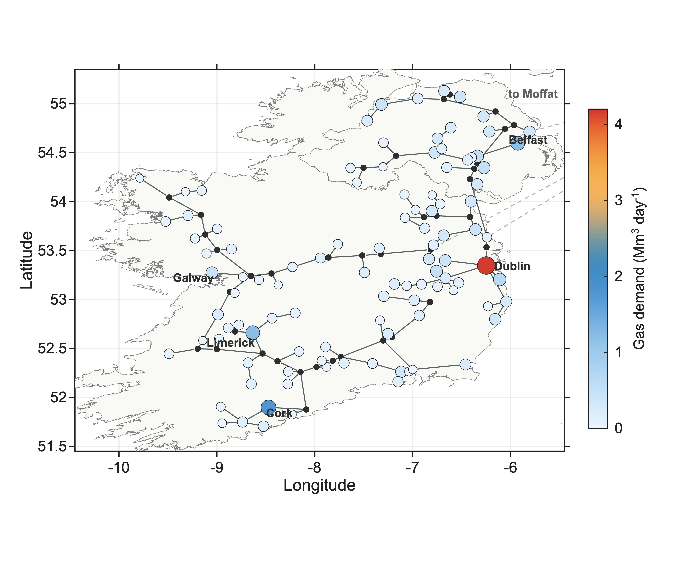
\includegraphics[width = 0.99\columnwidth]{figs/fig ireland gas system.pdf}
    \caption{Gas system on the island of Ireland. Node colour and size indicate daily gas demand, while small black dots denote gas nodes without assigned demand. Grey lines represent gas pipelines connecting gas nodes, and dashed grey lines indicate connections to the Moffat import node outside the displayed map extent.}
    \label{fig Ireland gas system}
\end{figure}

Fig. \ref{fig Ireland gas system} shows the schematic diagram of the gas system on the island of Ireland. The structure and physical parameters are provided by Gas Networks Ireland \cite{NetworkDevelopmentPlan}. It has 144 high-pressure gas nodes and gas pipelines operating above 16 barg. Currently, there are two major gas suppliers, including one from the UK (Moffat Point), with a maximum capacity of 35 Mm$^3$/day, and another from the northwest of Ireland (Corrib Point) with a maximum capacity of 6.21 Mm$^3$/day. Similar to the power system, the Dublin area has the largest gas consumption. Natural gas generally flows from northeast to southwest.

(1) Gas demand trend

Long-term and high-resolution gas demand is used for analysis. 
The hourly gas demand curve for a year is obtained from the Gas Networks Ireland data dashboard \cite{GasconsumptionbyMarketSector}.
The trends of gas demand in the future scenarios are predicted according to the Gas Forecast statement by Gas Networks Ireland \cite{GasForecastStatement2022, Irishelectricityandgasdemand}.
Gas demand is mainly from the power generation sector.
In the power sector, some coal-fired power plants (such as Moneypoint units) may retire in the future and be replaced by natural gas-generating units. In the meantime, with the 80\% renewable generation ambition from the Irish government's Climate Action Plan, the increasing renewable generation will replace the gas-fired generation. For industrial and commercial sectors, the gas demand will continue to increase in proportion to new connection numbers and Gross Domestic Product (GDP). For the residential sector, because Ireland's Climate Action Plan has explicitly banned the new installation of decentralised natural gas boilers from 2023 and replaced them with electric heat pumps, the gas demand will decrease in general. For the transportation sector, with the construction of new compressed natural gas (CNG) stations, the demand for natural gas is expected to grow.
Therefore, in summary, the gas demand will increase in the short term and reach a peak around 2025, and then continue to decrease from then on, as shown in Fig. \ref{fig future gas demand}. 

\begin{figure}
    \centering
    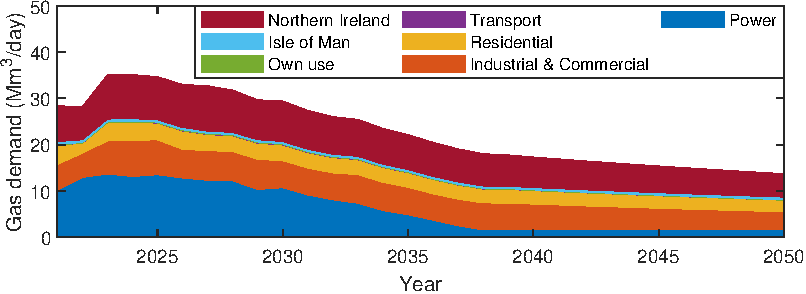
\includegraphics[width = 0.8\columnwidth]{figs/fig future ireland gas demand.pdf}
    \caption{Daily peak gas demand forecast for 2020 - 2050}
    \label{fig future gas demand}
\end{figure}

(2) Gas supply and demand models

Considering the use of alternative gases (hydrogen, biogas, etc.), the gas composition in the gas system cannot be regarded as constant. Seven gas components, which are commonly seen in natural gas, are considered, including methane, ethane, propane, butane, hydrogen, nitrogen, and carbon dioxide. Their gas compositions are denoted as $x_r$ ($r \in \mathcal{R}$), with $\sum_{r \in \mathcal{R}} x_r = 1$, where $\mathcal{R}$ is the set of gas components. For each different gas source (natural gas, biogas, etc.), the gas composition may differ. Then, the gas supply of a specific gas component can be calculated by:
\begin{gather}
    Q_{i,g,h,r}^{gs} = Q_{i,g,h}^{gs} x_{i,r}^{gs}
\end{gather}
where $Q_{i,g,h}^{gs}$ is the gas supply from source $g$ at gas node $i$; $x_{i,r}^{gs}$ is the gas composition of the supplied gas; and $Q_{i,g,h,r}^{gs}$ is the flow rate of gas component $r$ from this source.

Particularly for PTG, it uses water as a raw material and consumes electricity to produce hydrogen via the electrolysis process. Then, this process can be expressed as:
\begin{gather}
    Q_{i,g,h}^{ptg} = P_{i,g,h}^{ptg} \eta_{i,g}^{ptg} / GCV^{hy}
\end{gather}
where $Q_{i,g,h}^{ptg}$ is the hydrogen production rate of the PTG; $P_{i,g,h}^{ptg}$ is the power consumption of the PTG; $\eta_{i,g}^{ptg}$ is the electrolysis efficiency; $GCV^{hy}$ is the GCV of hydrogen.
The produced gas from PTG is assigned to the hydrogen component, so $Q_{i,g,h,\mathrm{hy}}^{ptg}=Q_{i,g,h}^{ptg}$ and the other component flows from PTG are zero.

For gas demand, considering different gas compositions, the total heat value of the supplied gas mixtures should match the gas demand. Therefore, we have:
\begin{gather}
    Q_{i,h,r}^{d} = x_{i,h,r} Q_{i,h}^{mix,d}, \quad
    \sum_{r \in \mathcal{R}} GCV_r Q_{i,h,r}^{d} = GCV^{ng} Q_{i,h}^{d}, \quad
    Q_{i,h,r}^{d} \geq 0
\end{gather}
where $GCV_r$ is the GCV of gas component $r$; $Q_{i,h,r}^{d}$ is the gas component $r$ consumed by the gas demand; $Q_{i,h}^{mix,d}$ is the total mixed-gas withdrawal that follows the nodal gas composition; $GCV^{ng}$ is the GCV of natural gas; and $Q_{i,h}^{d}$ is the gas demand expressed in gas flow rate.

(3) Gas network constraints

The produced gases are transported through pipelines. The physical properties of the gas flowing in a pipeline (gas pressure and gas flow rate) are governed by Weymouth equations \cite{an2003natural}:
\begin{gather}
    p_{i,h}^2 - p_{j,h}^2 = \gamma_{ij,h} \frac{16 F_{ij} (\rho^{ng})^2 T^{ng} L_{ij}z^{ng}}{\pi^2 D_{ij}^5} {R}_{ij} {Q}_{ij,h}^2
\label{eq gas flow weymouth} \\
     Q_{ij,h} = \sum_{r \in \mathcal{R}} Q_{ij,h,r}
\label{eq gas flow sum, gas constant} \\
    0 \leq Q_{ij,h} \leq Q_{ij}^{max}, \quad 0 \leq Q_{ij,h,r} \leq Q_{ij}^{max}
\label{eq capacity pipeline} \\
    p_i^{min} \leq p_{i,h} \leq p_i^{max}
\label{eq pressure limit}
\end{gather}
where $p_{i,h}$ is the gas pressure; $\gamma_{ij,h} \in \{-1,1\}$ is the direction of gas flow in pipeline $ij$, with $\gamma_{ij,h}=1$ denoting flow from node $i$ to node $j$; $F_{ij}$, $L_{ij}$, and $D_{ij}$ are the friction factor, length, and diameter of the pipeline, respectively; $\rho^{ng}$, $T^{ng}$, and $z^{ng}$ are the gas density, temperature, and compressibility factor of natural gas, respectively; $Q_{ij,h}$ is the non-negative gas-flow magnitude in the pipeline, and $Q_{ij,h,r}$ is the flow rate of gas component $r$; $Q_{ij}^{max}$ is the transmission capacity of the pipeline; $p_i^{min}$ and $p_i^{max}$ are the lower and upper bounds of nodal gas pressure, respectively.

During the transmission, multiple pipelines could be connected to the same gas node. The gases that flow into this node will be mixed evenly first and then distributed to the downstream pipelines. During this process, the nodal balance equations in terms of different gas components should be followed, as in (\ref{eq nodal gas balance}). The gas mixing process is expressed as (\ref{eq gas mixing}).
\begin{gather}
    \sum_{g\in \mathcal{G}_i^{gs}} {Q_{i,g,h,r}^{gs}} + \sum_{g \in \mathcal{G}_i^{ptg}}{Q_{i,g,h,r}^{ptg}}
    + \sum_{j \in \mathcal{J}_i}{\frac{1-\gamma_{ij,h}}{2} Q_{ij,h,r}} \notag \\
    = \sum_{j \in \mathcal{J}_i}{\frac{1+\gamma_{ij,h}}{2} Q_{ij,h,r} } +
    \sum_{g \in \mathcal{G}_i^{gpp}} Q_{i,g,h,r}^{gpp}
    + Q_{i,h,r}^{d}
\label{eq nodal gas balance} \\
    x_{i,h,r} = \bigg( \sum_{j \in \mathcal{J}_i} {\frac{1-\gamma_{ij,h}}{2} Q_{ij,h,r}}
    + \sum_{g\in \mathcal{G}_i^{gs}} {Q_{i,g,h,r}^{gs}}
    + \sum_{g\in \mathcal{G}_i^{ptg}} {Q_{i,g,h,r}^{ptg}} \bigg) /
\notag \\
    \bigg( \sum_{\hat r \in \mathcal{R}} \bigg( \sum_{j \in \mathcal{J}_i} {\frac{1-\gamma_{ij,h}}{2} Q_{ij,h,\hat r}}
    + \sum_{g\in \mathcal{G}_i^{gs}} {Q_{i,g,h,\hat r}^{gs}}
    + \sum_{g\in \mathcal{G}_i^{ptg}} {Q_{i,g,h,\hat r}^{ptg}} \bigg) \bigg)
\label{eq gas mixing}
\end{gather}
where $\mathcal{G}_i^{gs}$, $\mathcal{G}_i^{ptg}$ and $\mathcal{G}_i^{gpp}$ are the sets of gas sources, PTG units and gas-fired power plants at gas node $i$, respectively; and $\mathcal{J}_i$ is the set of pipelines connected to gas node $i$.

(4) Gas security constraints

When hydrogen is blended into the network and the gas composition changes, it may bring gas security issues. For example, appliances are usually designed and
tested at a given pressure with a specific type of gas. They
may not perform satisfactorily if the gas composition changes. The risks of flashback and fire hazards may also increase due to the higher flame speed of hydrogen. Therefore, certain gas security constraints should be imposed on the energy system operation to avoid too much hydrogen injection. According to recently amended Gas Safety (Management) Regulations \cite{GasSafetyRegulations}, the Wobbe index (WI), flame speed factor (FS) (which is additionally introduced to limit the flame speed), relative density, and the molar fraction of hydrogen can serve as indices to regulate gas safety:
\begin{gather}
    RD_{i,h} = \sum_{r \in \mathcal{R}} x_{i,h,r} M_r / M^{air}
\label{eq relative density} \\
    WI_{i,h} = \sum_{r \in \mathcal{R}} x_{i,h,r} GCV_r / \sqrt{RD_{i,h}}
\label{eq WI} \\
    FS_{i,h} = \frac{\sum_{r \in \mathcal{R}}{x_{i,h,r} fs_r }} {AF+5x_{i,h}^{ni}-18.8x_{i,h}^{ox}+1}
\label{eq FS} \\
    0 \leq x_{i,h}^{hy} \leq x^{hy,max}
\label{eq hydrogen fraction limit}\\
    RD_{i,h} \leq  RD^{max}
\label{eq relative density limit}\\
    WI^{min} \leq WI_{i,h} \leq WI^{max}
\label{eq WI limit}\\
    FS^{min} \leq FS_{i,h} \leq FS^{max}
\label{eq flame speed limit}
\end{gather}
where $RD_{i,h}$, $WI_{i,h}$, and $FS_{i,h}$ are the relative density, WI, and FS of the gas mixture at gas node $i$ in hour $h$, respectively; $M_r$ is the molecular weight of gas component $r$; $M^{air}$ is the molecular weight of air; $x_{i,h}^{hy}$, $x_{i,h}^{ni}$, and $x_{i,h}^{ox}$ are the molar fractions of hydrogen, nitrogen, and oxygen at gas node $i$ in hour $h$, respectively, with $x_{i,h}^{ox}=0$ for the gas mixtures considered here; $fs_r$ is the flame speed factor of gas component $r$; $AF$ is the air-fuel ratio; $x^{hy,max}$ and $RD^{max}$ are the upper bounds of hydrogen molar fraction and relative density, respectively; $WI^{min}$, $WI^{max}$, $FS^{min}$ and $FS^{max}$ are the lower and upper bounds of WI and FS, respectively.

\subsection{Solution method}

The formulated power-gas optimisation problem is nonlinear and nonconvex because of the gas-flow equations and gas-quality constraints. Following the solution strategy in \cite{wang2023optimal}, second-order cone relaxation and sequential programming are used to reformulate the nonlinear constraints into tractable conic subproblems. The resulting second-order cone programmes are solved with commercial solvers such as Gurobi or Mosek through the YALMIP modelling toolbox in MATLAB.


\section{International trading model and carbon emission impact analysis}

\subsection{Demand and supply models of hydrogen and ammonia}

International hydrogen and ammonia trading can help balance the uneven distribution of offshore hydrogen and ammonia production potential across countries. It also supports a cost-minimising allocation for Europe-wide decarbonisation. Modelling production capacity and demand is therefore a prerequisite for deriving Europe's future international hydrogen trading landscape. Among the studied countries, Germany has officially announced future hydrogen import needs. Around 90--110 TWh yr$^{-1}$ of hydrogen will be needed by 2030, but the offshore/onshore renewable hydrogen generation capacity will only be 5 GW by then, which accounts for 12.73\%--15.56\% of the total hydrogen demand. Even with an additional 5 GW added by 2035 or 2040, Germany still needs considerable hydrogen imports \cite{NationalHydrogenStrategyGermany}. Belgium is another country that has clearly announced hydrogen import needs. The import of renewable molecules for Belgium will amount to between 3 and 6 TWh in 2030 and between 100 and 165 TWh in 2050, in order to satisfy domestic demand. The import solutions are estimated to be more cost-efficient than local production \cite{GreenHydrogenState}. The demand projection from the European Hydrogen Backbone is used, as shown in Fig. \ref{fig hydrogen demand} \cite{Analysingfuturedemand}.

\begin{figure}
    \centering
    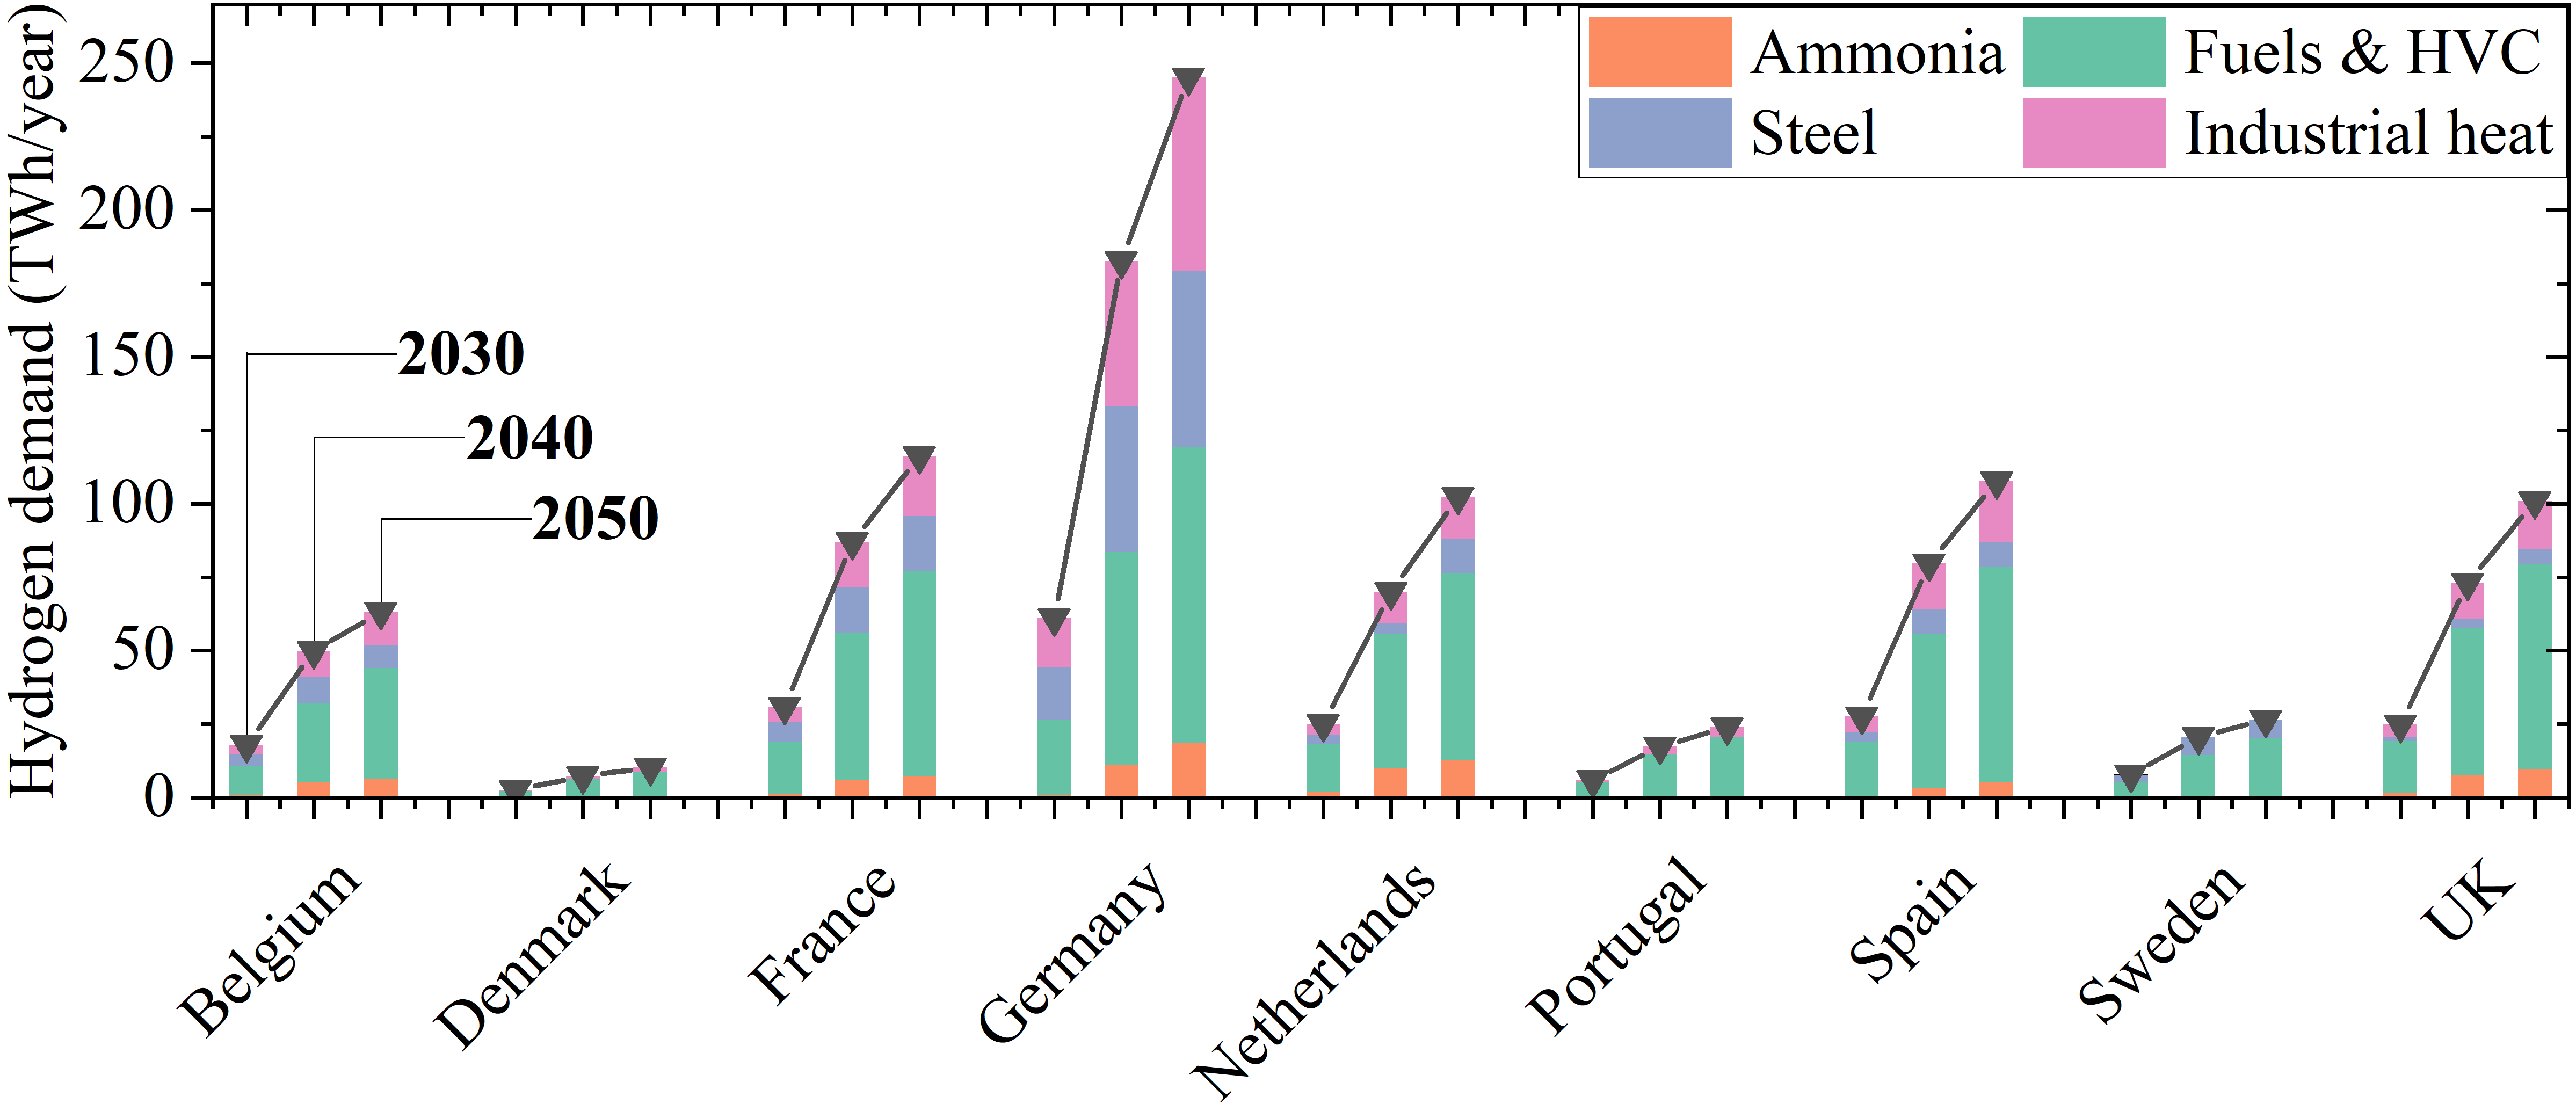
\includegraphics[width = 0.99\columnwidth]{figs/fighydrogendemand2.png}
    \caption{Projected hydrogen and ammonia demand for coastal European countries.}
    \label{fig hydrogen demand}
\end{figure}

\begin{table}[tbp]
\centering
\caption{Offshore wind capacity in European countries (GW)}
\label{tab owf capacity}
\begin{tabular}{llll}
\hline
               & 2030       & 2040       & 2050      \\ \hline
Belgium        & 6 \cite{NSOG}       & 8 \cite{NSOG}         & 8 \cite{NSOG}         \\
Denmark        & 9 \cite{Offshorewindfarmstenderedtowards2030}          & 10 \cite{EnergyIslandintheNorthSea}        & 35 \cite{NSOG}       \\
France         & 18 \cite{FrancepassesRenewable}        & 20 (estimated)         & 40 \cite{Francecommitsto40}       \\
Germany        & 30 \cite{Morewindenergyatsea}        & 40 \cite{Morewindenergyatsea}        & 70 \cite{Morewindenergyatsea}       \\
Ireland        & 5 \cite{FutureFrameworkforOffshoreRenewableEnergy}         & 20 \cite{FutureFrameworkforOffshoreRenewableEnergy}        & 37 \cite{FutureFrameworkforOffshoreRenewableEnergy}       \\
Netherlands    & 21 \cite{Offshorewindenergy}       & 50 \cite{NetherlandsSets70GW}        & 70 \cite{NetherlandsSets70GW}        \\
Norway         & 3  \cite{300GWNorthSea}        & 22 \cite{ENERGYTRANSITIONNORWAY2023}        & 43 \cite{ENERGYTRANSITIONNORWAY2023}       \\
Portugal       & 10 \cite{Portugaltolaunch}        & 10 \cite{Atlantic}        & 10 \cite{Atlantic}       \\
Spain          & 3  \cite{Spainissuesplan}        & 10 (estimated)          & 17 \cite{Spainrepresents}        \\
Sweden         & 3  \cite{FinlandDenmarkSweden}        & 11 (estimated) \cite{Roadmap2040}         & 41 \cite{Offshorewinddevelopment}       \\
United Kingdom & 55  \cite{Offshorewindnetzero}       & 80 \cite{Offshorewindnetzero}        & 125 \cite{Offshorewindnetzero}      \\ \hline
\end{tabular}
\end{table}

The offshore wind capacity of each country is listed in Table \ref{tab owf capacity}. The reference for each value is given. Most of the numbers are obtained from official offshore wind development plans from governments. For those countries without clear written plans, we use the numbers from the latest EU non-binding agreement or press releases by their governments. We assume that 10\% of the export-available hydrogen capacity can be routed to ammonia production. This is treated as a conservative ammonia-route capacity assumption, rather than a policy target, and is supported by the International Renewable Energy Agency (IRENA) outlook in which ammonia shipping is identified as a major route for internationally traded hydrogen by 2050 \cite{IRENAGlobalHydrogenTradeOutlook2022}. These capacities first set the gross offshore hydrogen production potential in a country. The part already absorbed by the domestic power and gas systems is deducted before the remaining supply is made available for export. We denote the domestic hydrogen absorption as:
\begin{align}
    Q_{ic}^{hy,abs} = \sum_{i \in \mathcal{I}_{ic}^E} \sum_{g \in \mathcal{G}_i^{ptg}} \sum_{h=1}^{8760} Q_{i,g,h}^{hy}
\end{align}
Then, the available hydrogen export capacity $Q_{ic}^{hy,ex,max}$ can be calculated as:
\begin{align}
    Q_{ic}^{hy,ex,max} = \max \left\{0,\; \left(8760 P_{ic}^{owf,max} CF_{ic} - E_{ic}^{owf,dom}\right) \eta^{ptg} - Q_{ic}^{hy,abs} \right\}
\end{align}
The corresponding ammonia export capacity is defined as:
\begin{align}
    Q_{ic}^{am,ex,max} = \alpha^{am} \eta^{asr} Q_{ic}^{hy,ex,max}
\end{align}
where $\mathcal{I}_{ic}^E$ is the set of electricity-system nodes located in country $ic$; $Q_{i,g,h}^{hy}$ is the hydrogen energy supplied by PTG facility $g$ at node $i$ to the domestic energy system during hour $h$, excluding hydrogen exports; $E_{ic}^{owf,dom}$ is the annual offshore wind electricity used directly to meet domestic electricity demand, excluding electricity used for electrolysis, expressed in MWh yr$^{-1}$; $P_{ic}^{owf,max}$ is the total offshore wind capacity for country $ic$, expressed in MW in the calculation; $CF_{ic}$ is the average capacity factor for country $ic$; $\eta^{ptg}$ is the electrolyser efficiency; $\alpha^{am}=0.1$ is the share of export-available hydrogen capacity routed to ammonia production; $\eta^{asr}$ is the ammonia synthesis efficiency; and the factor 8760 converts installed capacity into annual energy output. Offshore wind capacities reported in GW in Table \ref{tab owf capacity} are converted to MW before applying these equations.

\subsection{Optimal international trading model}

The optimal international trading model determines the hydrogen and ammonia flows among European countries. The optimisation objective is to minimise the total external cost ($C^{ex}$), including European offshore production cost ($C^{prod}$), transportation cost ($C^{trans}$), and delivered import cost ($C^{im}$) from distant countries or regions during international hydrogen and ammonia trading.
\begin{align}
    \min C^{ex} & = C^{prod} + C^{trans} + C^{im}
    \notag \\
    & = \sum_{ic \in \mathcal{CT}} \left[
    f^{hy,prod}\left(Q_{ic}^{hy,spl}\right)
    + f^{am,prod}\left(Q_{ic}^{am,spl}\right)
    \right]
     \notag\\
     & + \sum_{ip \in \mathcal{PT}} \sum_{jp \in \mathcal{PT}}^{jp \neq ip}
     \left(C_{ip,jp}^{trans,hy} + C_{ip,jp}^{trans,am}\right)
     \notag\\
     & + \rho^{im,hy} \sum_{ic \in \mathcal{CT}}Q_{ic}^{hy,im}
     + \rho^{im,am} \sum_{ic \in \mathcal{CT}}Q_{ic}^{am,im}
\end{align}
where $ic$ is the index for countries and $ip$, $jp$ are the indices for ports; $\mathcal{CT}$ and $\mathcal{PT}$ are the sets of countries and ports, respectively; $f^{hy,prod}$ and $f^{am,prod}$ are the piecewise production cost functions fitted from the European offshore hydrogen and ammonia cost-supply curves in Section \ref{sec cost}, respectively; $Q_{ic}^{hy,spl}$ and $Q_{ic}^{am,spl}$ are the hydrogen and ammonia production from country $ic$, respectively; $C_{ip,jp}^{trans,hy}$ is the total shipping cost in the shipping line that links port $ip$ and $jp$; $\rho^{im,hy}$ and $\rho^{im,am}$ are the delivered unit costs of internationally imported hydrogen and ammonia, respectively; $Q_{ic}^{hy,im}$ and $Q_{ic}^{am,im}$ are the quantities of import hydrogen and ammonia for country $ic$, respectively.

The model is subject to:

(1) Supply and demand constraints:

Export-available offshore hydrogen can either be supplied as hydrogen or converted to ammonia. The combined hydrogen-equivalent supply must be within the available hydrogen export capacity, as in (\ref{eq offshore production hydrogen cons}). The ammonia supply is further limited by the available ammonia export capacity in (\ref{eq offshore production ammonia cons}). Equations (\ref{eq country hydrogen balance cons}) and (\ref{eq country ammonia balance cons}) model the country-level supply-demand balance for hydrogen and ammonia, respectively.
\begin{gather}
    0 \leq Q_{ic}^{hy,spl} + Q_{ic}^{am,spl} (\eta^{asr})^{-1} \leq Q_{ic}^{hy,ex,max}
\label{eq offshore production hydrogen cons}\\
    0 \leq Q_{ic}^{am,spl} \leq Q_{ic}^{am,ex,max}
\label{eq offshore production ammonia cons}\\
    Q_{ic}^{hy,spl} - \sum_{ip \in \mathcal{PT}_{ic}} \sum_{jp \in \mathcal{PT}}^{jp \notin \mathcal{PT}_{ic}} \left( Q_{ip,jp}^{hy,trans} + Q_{ip,jp}^{hy,route} \right) - Q_{ic}^{hy,dm} + Q_{ic}^{hy,im}= 0
\label{eq country hydrogen balance cons}\\
    Q_{ic}^{am,spl} - \sum_{ip \in \mathcal{PT}_{ic}} \sum_{jp \in \mathcal{PT}}^{jp \notin \mathcal{PT}_{ic}} \left( Q_{ip,jp}^{am,trans} + Q_{ip,jp}^{am,route} \right) - Q_{ic}^{am,dm} + Q_{ic}^{am,im}  = 0
\label{eq country ammonia balance cons}
\end{gather}
where $\eta^{asr}$ is the efficiency of the ammonia synthesis reactor; $Q_{ic}^{am,ex,max}$ is the export capacity of ammonia for country $ic$; $\mathcal{PT}_{ic}$ is the set of ports located in the country $ic$; $Q_{ip,jp}^{hy,trans}$ and $Q_{ip,jp}^{am,trans}$ are the annual hydrogen and ammonia shipped from port $ip$ to $jp$, respectively; $Q_{ip,jp}^{hy,route}$ and $Q_{ip,jp}^{am,route}$ are the annual fuel (hydrogen or ammonia) consumptions of all ships operating on the route between port $ip$ and $jp$, respectively; $Q_{ic}^{hy,dm}$ and $Q_{ic}^{am,dm}$ are the domestic hydrogen and ammonia for country $ic$, respectively.

(2) Transportation costs and constraints:

The transportation cost for a shipping line includes annualised ship investment and operation and maintenance costs. Fuel consumed during shipping is represented separately by the route fuel terms in the country balance constraints. For a specific ship, given the annual operating hours ($T^{op}$), the number of trips in a year ($n^{trip}$) can be calculated as:
\begin{gather}
    n_{ip,jp}^{trip} = \frac{T^{op}}{2(T_{ip,jp}^{tv} + T^{ld})}
\\
    T_{ip,jp}^{tv} = L_{ip,jp} / v^{ship}
\end{gather}
where $T_{ip,jp}^{tv}$ and $T^{ld}$ are the travelling time and load/unload time; $L_{ip,jp}$ is the distance along the shipping line between port $ip$ and $jp$; $v^{ship}$ is the velocity of ships.

The country-wide average unit fuel cost of shipping hydrogen is shown in Fig. \ref{fig ship cost}. The cost depends on the shipping route lengths, which can be obtained from SeaRates \cite{SeaRates}. Considering the approximately 60 \texteuro{} MWh$^{-1}$ marginal price for hydrogen, the transportation fuel cost accounts for around 0.08\%--2.12\%. From Fig. \ref{fig ship cost}a to Fig. \ref{fig ship cost}c, the fuel cost generally declines as hydrogen production costs decrease. Among different shipping routes, those connected to Portugal, such as Sweden--Portugal and Norway--Portugal, have relatively higher costs because of the longer shipping distances.

\begin{figure}
    \centering
    
\includegraphics[width = 0.95\columnwidth]{figs/fig shipping fuel cost.pdf}
    \caption{Route-level fuel cost for liquid-hydrogen shipping in 2030, 2040 and 2050. Grey diagonal cells indicate non-applicable within-country routes.}
    \label{fig ship cost}
\end{figure}


The total capacity per year of a port-to-port shipping line, and its fuel consumption can be calculated as:
\begin{gather}
    Q_{ip,jp}^{hy,trans,max} = Q_{ip,jp}^{hy,ship,max} n_{ip,jp}^{trip} n_{ip,jp}^{hy,ship}
\label{eq hy ship flow} \\
    Q_{ip,jp}^{am,trans,max} = Q_{ip,jp}^{am,ship,max} n_{ip,jp}^{trip} n_{ip,jp}^{am,ship}
\label{eq am ship flow} \\
    \left| Q_{ip,jp}^{hy,trans} \right| \leq  Q_{ip,jp}^{hy,trans,max}
\label{eq hy ship cap} \\
    \left| Q_{ip,jp}^{am,trans} \right| \leq  Q_{ip,jp}^{am,trans,max}
\label{eq am ship cap} \\
    Q_{ip,jp}^{hy,route} = 2 n_{ip,jp}^{trip} T_{ip,jp}^{tv} Q^{hy,ship} n_{ip,jp}^{hy,ship}
\label{eq hy ship fuel} \\
    Q_{ip,jp}^{am,route} = 2 n_{ip,jp}^{trip} T_{ip,jp}^{tv} Q^{am,ship} n_{ip,jp}^{am,ship}
\label{eq am ship fuel}
\end{gather}
where $Q_{ip,jp}^{hy,trans,max}$ and $Q_{ip,jp}^{am,trans,max}$ are the maximum hydrogen and ammonia transportation capacities between port $ip$ and $jp$, respectively; $Q_{ip,jp}^{hy,ship,max}$ and $Q_{ip,jp}^{am,ship,max}$ are the hydrogen and ammonia storage capacities per ship, respectively; $n_{ip,jp}^{hy,ship}$ and $n_{ip,jp}^{am,ship}$ are the numbers of invested hydrogen and ammonia transportation ships between port $ip$ and $jp$, respectively; they are the decision variables in the optimisation problem; $Q^{hy,ship}$ and $Q^{am,ship}$ are the operating hydrogen and ammonia fuel consumptions per ship per hour, respectively.

The annualised cost of each shipping line is:
\begin{align}
    C_{ip,jp}^{trans,hy} =  n_{ip,jp}^{hy,ship} \left( \frac{C^{cap,hy,ship}}{\sum_{\tau = 1}^{T^{ship}} (1+r)^{-\tau}} + C^{om,hy,ship} \right)
    \\
    C_{ip,jp}^{trans,am} =  n_{ip,jp}^{am,ship} \left( \frac{C^{cap,am,ship}}{\sum_{\tau = 1}^{T^{ship}} (1+r)^{-\tau}} + C^{om,am,ship} \right)
\end{align}
where $C^{cap,hy,ship}$ and $C^{cap,am,ship}$ are the capital costs of hydrogen and ammonia ships, respectively; $C^{om,hy,ship}$ and $C^{om,am,ship}$ are the corresponding annual operation and maintenance costs; $T^{ship}$ is the lifespan of the ship.

(3) Solution method

Due to the discontinuity of the hydrogen and ammonia cost-supply curves, the original problem is formulated as a mixed integer linear programming problem and solved by the Gurobi \cite{Gurobi} commercial solver via the YALMIP modelling toolbox in MATLAB.

\subsection{Carbon-mitigation accounting}

Carbon mitigation is calculated after solving the international trading model. The metric is a direct displacement-accounting value, rather than a full lifecycle assessment. Hydrogen and ammonia quantities are represented as annual delivered energy in the trade model. For a demand country $ic$, the annual avoided carbon dioxide emissions are calculated as:
\begin{align}
    M_{ic}^{hy} &=
    Q_{ic}^{hy,dm} EF^{hy}
    \\
    M_{ic}^{am} &=
    Q_{ic}^{am,dm} EF^{am}
    \\
    M_{ic} &= M_{ic}^{hy} + M_{ic}^{am}
\end{align}
where $Q_{ic}^{hy,dm}$ and $Q_{ic}^{am,dm}$ are the annual delivered hydrogen and ammonia energy demands from the trade model, expressed in MWh yr$^{-1}$; $EF^{hy}$ is the avoided CO$_2$ emission factor per unit of delivered hydrogen energy relative to natural gas displacement; and $EF^{am}$ is the avoided CO$_2$ emission factor per unit of delivered ammonia energy relative to the reference production or utilisation pathway. Both emission factors are expressed in kg CO$_2$ MWh$^{-1}$. For example, displacing natural gas represented as methane on an equal-energy basis, with a lower heating value of 50 MJ kg$^{-1}$, gives $EF^{hy}=198$ kg CO$_2$ MWh$^{-1}$ from direct combustion emissions. Consistent unit conversions are applied to report emissions in Mt CO$_2$ yr$^{-1}$.

Supplier-attributed carbon mitigation is then assigned according to the optimised delivery matrix. Hydrogen and ammonia delivered from supplier $ic$ to demand country $jc$ are converted into avoided carbon dioxide emissions using the corresponding demand-country accounting factors. International imports are treated as imported low-carbon hydrogen and ammonia that meet the same final demand, and are assigned to an additional international-import row. Domestic self-supply is assigned on the diagonal as the residual mitigation after imported supplier contributions are subtracted:
\begin{align}
    A_{ic,ic} = M_{ic} - \sum_{r \neq ic} A_{r,ic}.
\end{align}
The total mitigation reported in the main manuscript is $\sum_r \sum_{ic} A_{r,ic}$. The European offshore contribution excludes the international-import row and is therefore lower than total mitigation whenever external imports meet part of the demand. The accounting values used in the main manuscript are summarised in Table \ref{tab carbon accounting summary}.

\begin{table}[tbp]
\centering
\caption{Carbon-mitigation accounting values used in the main manuscript. Total mitigation includes the international-import node when present. European offshore contribution excludes the international-import node.}
\label{tab carbon accounting summary}
\begin{tabular}{lrrr}
\hline
Metric & 2030 & 2040 & 2050 \\ \hline
Total mitigation (Mt CO$_2$ yr$^{-1}$) & 43.46 & 129.77 & 175.50 \\
European offshore contribution (Mt CO$_2$ yr$^{-1}$) & 43.46 & 103.19 & 158.30 \\
International-import contribution (Mt CO$_2$ yr$^{-1}$) & 0.00 & 26.58 & 17.20 \\
International hydrogen import (TWh yr$^{-1}$) & 0.00 & 116.20 & 62.20 \\ \hline
\end{tabular}
\end{table}





%%===========================================================================================%%
%% If you are submitting to one of the Nature Portfolio journals, using the eJP submission   %%
%% system, please include the references within the manuscript file itself. You may do this  %%
%% by copying the reference list from your .bbl file, paste it into the main manuscript .tex %%
%% file, and delete the associated \verb+\bibliography+ commands.                            %%
%%===========================================================================================%%

\bibliography{sn-bibliography}% common bib file
%% if required, the content of .bbl file can be included here once bbl is generated
%%\input sn-article.bbl


\end{document}
